%!TEX encoding = UTF-8 Unicode
\documentclass[12pt, twoside, a4paper]{report}

% To format double quotes in the right way
\usepackage[autostyle=false, style=english]{csquotes}
\MakeOuterQuote{"}

\usepackage{algorithm2e}% http://ctan.org/pkg/algorithms
\usepackage{algpseudocode}% http://ctan.org/pkg/algorithmicx

\usepackage[utf8]{inputenc}

\usepackage{cite}
\usepackage{fancyhdr}
\usepackage{lipsum}
\usepackage{graphicx}
\usepackage[labelfont=bf]{caption}
\usepackage{amsfonts}
\usepackage{amsmath}
\usepackage{chngcntr}
\usepackage{tabularx}
\usepackage{multirow}
\usepackage{hyperref}
\hypersetup{
	colorlinks,
	citecolor=black,
	filecolor=black,
	linkcolor=black,
	urlcolor=black
}
\usepackage{pdfpages}
\usepackage{booktabs}
\usepackage{subcaption}
\usepackage[space]{grffile}

\counterwithout*{footnote}{chapter}
\pagestyle{fancy}
\fancyhf{}
\renewcommand{\headrulewidth}{0.01pt}
\fancyhead[LE,RO]{\thepage}
\fancyhead[LO]{\leftmark}
%\fancyhead[RE,LO]{\leftmark}
\fancyhead[RE]{\rightmark}
%\fancyfoot[CE,CO]{\thepage}
\newcommand{\whitepage}{\clearpage
						\thispagestyle{empty}
						\phantom{a}
						\vfill}

\begin{document}

% Include the title page
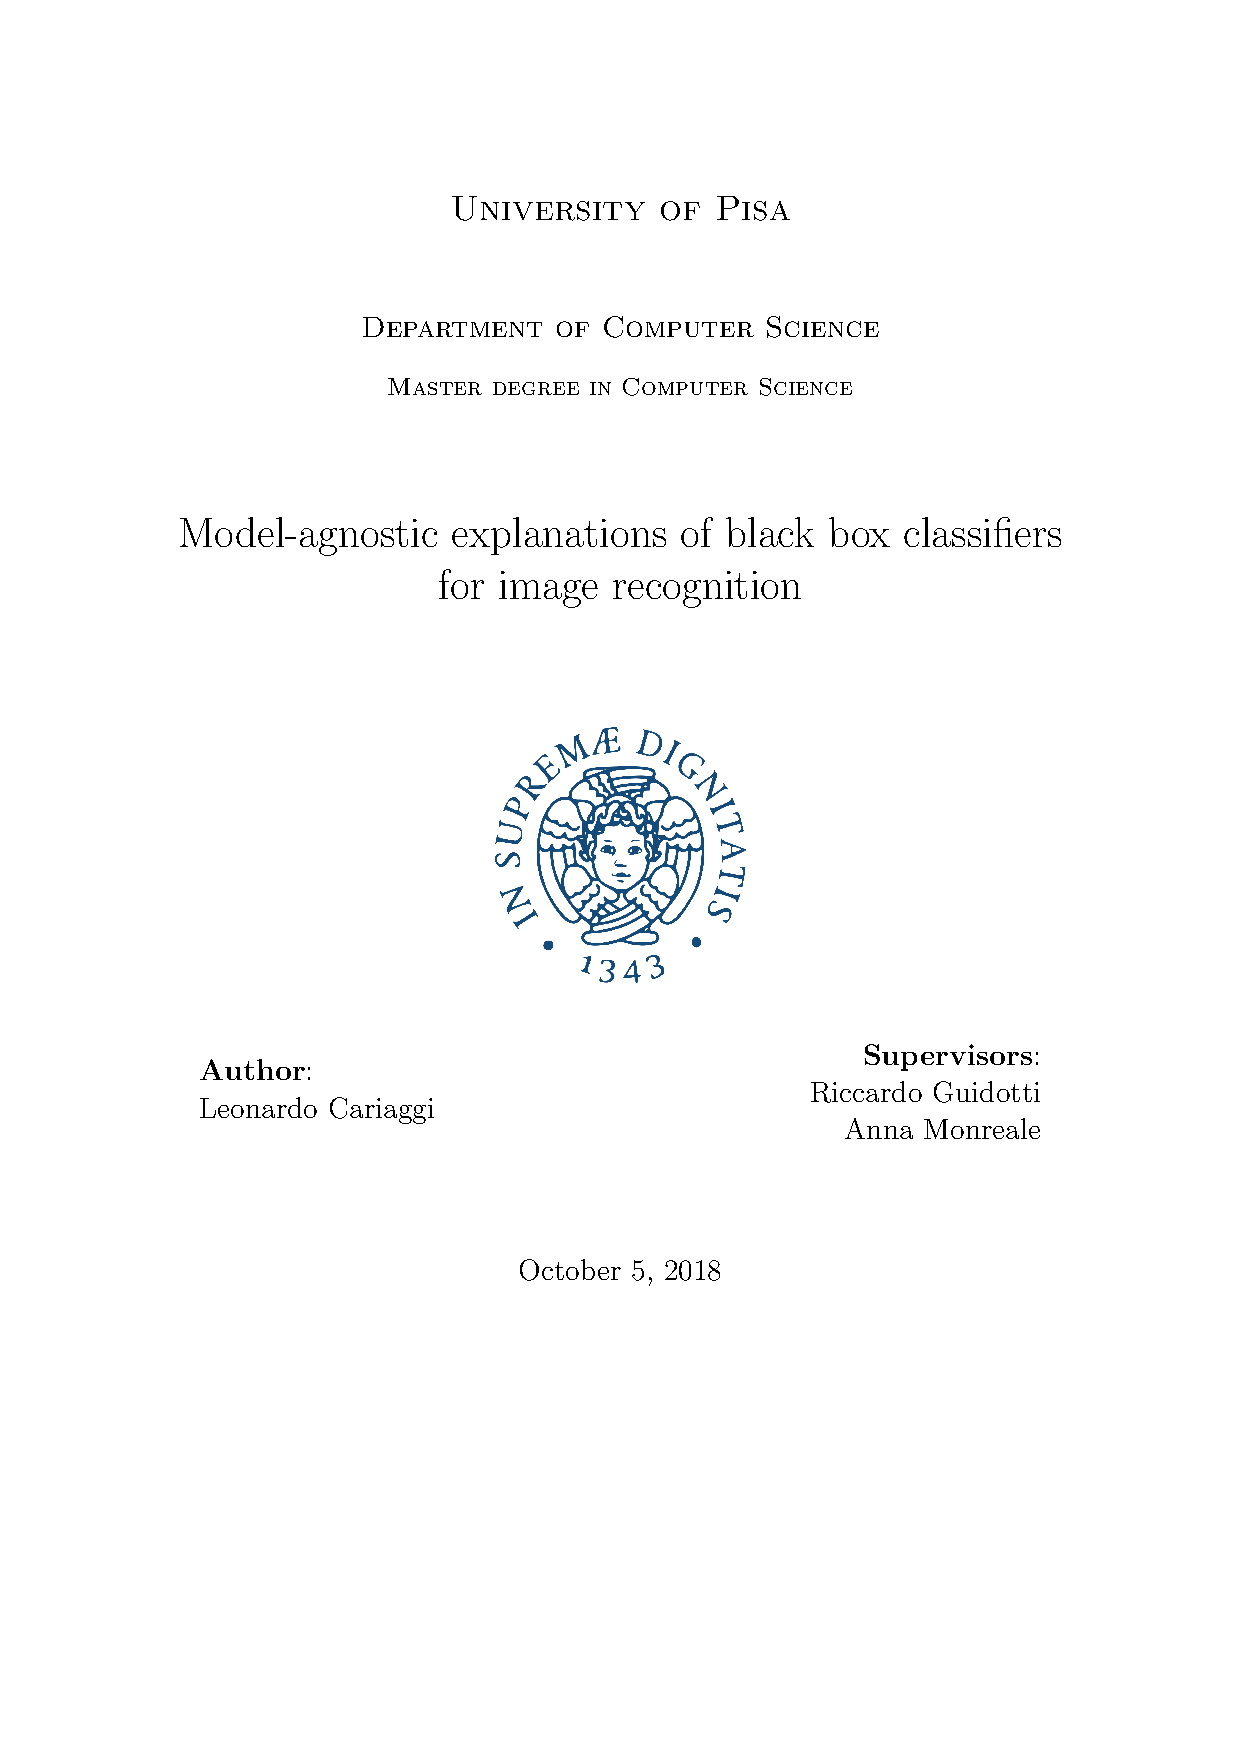
\includepdf{thesis_cover/cover.pdf}

\whitepage

\sloppy
\nocite{*}

\newpage

\chapter*{Ringraziamenti}

\thispagestyle{empty}
\footnotesize

Vorrei ringraziare i miei relatori, Anna Monreale e Riccardo Guidotti, che hanno saputo fin da subito consigliarmi e farmi iniziare col piede giusto l'ultimo capitolo della mia carriera di studente universitario. Grazie della fiducia, della motivazione, dell'appoggio e dell'entusiasmo che mi avete sempre trasmesso durante l'ultimo semestre.

Agli amici e compagni di gioco dello Star: grazie per gli innumerevoli sabati passati insieme, per le partite, per i confronti, le discussioni e le risate. La facilità e la naturalezza con la quale stringevamo amicizia mi riportava sempre indietro nel tempo. In ordine casuale ringrazio Fili, Michelangelo, Fla, Acco, Geno, F. Donati, Cacio, T. Conti, Ono, Topini, Mirko, E. Cassai, Crucio, Fonta, Bernini e tutti gli altri. 

Grazie anche ai miei amici di lunga data, Uri, Ale e Boa, con i quali ho sempre passato (e passerò ancora) momenti di gioia e spensieratezza. Grazie Iulian, sei sempre rimasto lo stesso dai tempi della 3 INF: un amico sincero e vero.
Grazie anche a tutti i miei amici di infanzia: in vostra compagnia ho trascorso molti dei migliori anni della mia vita.

Grazie agli amici dell'università, compagni di corso e ai ragazzi del mio ufficio. 
Grazie a te Tri, che mi hai dimostrato che, con un incessante impegno e una buona dose di volontà, si può anche girare il mondo alla nostra età. Grazie allo chef, a Qiong, a Vân, Anh, Helen, Lin e a tutti i tuoi amici per aver condiviso con me le vostre esperienze.

Ai migliori coinquilini che potessi avere, Matteo, Gianluca e Andrea, voglio augurare il meglio: grazie per aver reso piacevole la mia permanenza a Pisa e per avermi insegnato tante cose.

Grazie a Luciana, per la tua gentilezza e la tua semplicità e per aver reso una delle mie ultime sessioni estremamente più leggera e tranquilla. Abbiamo condiviso il nostro percorso di studio soltanto nell'ultimo semestre, ma mi auguro che continueremo a tenerci in contatto. 

Un sincero grazie a Giulia, indubbiamente la persona più riconoscente e generosa che conosca: quelli che per te sono gesti naturali e spontanei hanno avuto e continuano ad avere per me un significato enorme. Grazie per il tempo che abbiamo condiviso, spero davvero che ci sarà ancora l'occasione di vederci o sentirci e di fare un viaggio nel tanto desiderato Giappone.

Grazie dunque anche alla mia professoressa di giapponese, Yukari Saitō, che ha reso ancora più grande il mio interesse verso quest'affascinante lingua e mi ha appoggiato durante tutto il percorso.

Grazie infine alla mia famiglia, che mi ha sempre sostenuto e ha reso possibile tutto questo.

\whitepage
\newpage

\chapter*{Acknowledgements}
\thispagestyle{empty}

I would like to thank my supervisors, Anna Monreale and Riccardo Guidotti, who gave me suggestions and made me start the last chapter of my student's career in the best way. Thank you for your trust, motivation, help and enthusiasm.

To the friends and mates of the Star: thank you for the countless Saturdays spent together, for the matches, the confrontations, the discussions and the funny moments. We became friends in such an easy and natural way that reminded me of the good old times. I would like to thank, in random order, Fili, Michelangelo, Fla, Acco, Geno, F. Donati, Cacio, T. Conti, Ono, Topini, Mirko, E. Cassai, Crucio, Fonta, Bernini and everyone else.

Thanks to my friends Uri, Ale and Boa, with whom I always spent (and will spend) moments of happiness. Thank you Iulian, you have always stayed the same from the times of high school: a real and sincere friend. Thanks to all the friends of my childhood: with you I have spent many of the best years of my life. 

Thanks to the friends I met at the university, classmates and office mates. Thank you Tri, because you showed me that, with enough self-confidence and will power, nothing can stop us from traveling around the world. Thanks to the chef, to Qiong, to Vân, Anh, Helen, Lin and all your friends for sharing your stories with me.

To the best housemates ever, Matteo, Gianluca and Andrea, I would like to wish the best: thank you for the nice years spent in Pisa and for the things you taught me. 

Thank you Luciana, for your kindness and simplicity and for making my last exam session extremely light and peaceful. We shared our studies just for the last semester, but I hope we will always keep in touch. 

Thank you Giulia, you are unarguably the most grateful and generous person I know: all the actions and manners that you find normal meant and continue to mean a lot to me. Thank you for the time we shared, I really hope we will meet and keep in touch again and travel together to Japan.

Also, I would like to thank my Japanese teacher Yukari Saitō, that made my interest for this fascinating language even bigger and always supported me during the whole program. 

Finally I would like to thank my family, who always helped me and made everything possible.

\whitepage
\normalsize
\tableofcontents

\chapter{Introduction}

In the last years, automated decision systems have been widely used in all those situations in which classification, recognition and prediction tasks were the main concern. All these systems exploit machine learning techniques to extract the possible relationships between what we give them as input and what we expect as output. Input variables can be of any type, as long as it is possible to find a convenient representation for them. For instance we can think of images as matrices of pixels or even as a set of features (that, intuitively, correspond to specific areas or patterns of the image). 

In other cases, we may need to deal with data that somehow represent a collection of information about people, products or any other thing we can think of. This type of data is called tabular data. In addition, machine learning techniques can be applied to text data: in these situations, a convenient representation might be the frequency of words inside a document.

We talk about "Black boxes" when dealing with classifiers having an opaque, hidden internal structure whose comprehension is not our main concern. What we are trying to understand in this work are, instead, the reasons that lead classifiers to make certain predictions. Models are built through the so-called learning phase, using large amounts of data as training instances. These might include sensible information such as credit card numbers, health status, locations and so on, so it is fundamental to ensure they are used properly to avoid any kind of discrimination and, in general, unfair usage. 

On 25 May 2018, the European Parliament approved the \textit{General Data Protection Regulation} (GDPR) on data protection and privacy for all the citizens living in the European Union (EU) and the European Economic Area (EEA). It addresses the export of personal data outside the EU and EEA areas, giving people control over their personal data. On top of that, there are also restrictions and guidelines that companies (or any other organization holding personal data) are forced to follow: for instance, data must be stored using pseudonymization or full anonymization and use the highest-possible privacy settings by default, so that the data is not available publicly without explicit, informed consent, and cannot be used to identify a subject without additional information stored separately.
An innovative aspect of the GDPR, which has been much debated, are the clauses on automated individual decision-making processes (prediction models in this case) which, for the first time, introduce a right of explanation for all individuals to obtain meaningful explanations of the logic involved when automated decision making takes place.

Another reason why we are interested in explanations derives from the fact that we constantly use decision systems that we cannot understand. Typically, our main concern is the maximization of the model's performances (not caring at all about what happens under the hood). What can we do when we obtain relatively bad results and/or unexpected behaviors? Also, how can we prove that an image classifier built to recognize poisonous mushrooms actually focuses on the mushrooms themselves and not on the background?
If we take an \textit{Artificial Neural Network} (ANN) as an example, trying to understand the decision process is just hopeless (because what we have is just a huge set of real numbers in the weight matrix). 
There are, of course, models that can be completely understood (Decision Trees, rule-based models), but in general it has been observed that they are less performant. So, rather than trying to "open" the black boxes, we focus just on the predictions themselves. Our goal is now to understand predictors \textit{a-posteriori} and comprehend \textit{what} the black box has learned and \textit{how} it learned it \cite{fong}.

For the specific case of image data, explanations are even more necessary. This is because users expect the model to make right decisions on the basis of interesting, comprehensible facts and not by luck/chance. If we think for instance of medical diagnosis \cite{healthcare}, machine learning models might be used to predict whether a patient has a certain disease just by looking at his/her x-rays scan. In such a critical situation we must ensure that the classifier looks at specific internal organs and/or bones to make its prediction, not focusing on irrelevant details (i.e. background, text annotations). 
The whole point of explanations is not to make the model perform better, but rather to let users trust it: an accuracy of 100\%, in fact, does not always imply that the model has learned the target concept.

Explanation of predictions on images can be obtained by finding regions whose deletion causes the classification score of a fixed label to drop significantly. This is because we genuinely expect that the model's prediction does not change at all as we remove useless, uninformative patches. 
Such patches can be either extracted by an iterative process or even by training a model that predicts it given the class label \cite{real_time_image_saliency}. 

\bigskip

In this work we make several contributions. First, we propose a framework of explanations as sparse linear models trained on \textit{Interpretable Data Represetations} (extending LIME \cite{lime}). Then, we list some of the possible drawbacks of LIME and propose different workarounds. We also experiment the impact of clustering algorithms on the definition of informative regions and the overall quality of the explanations on a test set of 1000 images (from the ILSVRC2012 dataset \cite{ilsvrc}). 
Finally, we also introduce a systematic approach for the evaluation of explanations, creating an annotated data set that contains the optimal regions that explanations should cover for each of the images in the test set.

The rest of this work is organized as follows. In Chapter \ref{chapt:related-work} we give an overview of the current state-of-art methods for explaining predictions in image classification. We also analyze different strategies for image data representation. Next, in Chapter \ref{chapt:background} we present this work's starting point and discuss all the logic behind it in detail. In Chapter \ref{chapt:approach} we then present the general structure of our work and propose various extensions to the original approach, motivating our choices. In Chapter \ref{chapt:experiments} we validate our approach through experiments (by picking a test set of 1000 images) and compare the obtained results. Finally, in Chapter \ref{chapt:conclusions} we summarize all the aspects of our solution and draw the conclusions, also indicating future research directions.

\whitepage


\chapter{Related work}\label{chapt:related-work}

This chapter will be dedicated to a general overview of the state-of-the-art methods that explain the predictions of a black box on images. According to the type of explanation that we want to build, we have to distinguish between different cases. 

The first kind of approaches aim at capturing the \textit{global} logic of a black box by building an interpretable model that is able to mimic its behaviour for any input instance. We refer to this problem as \textit{Black Box Model Explanation} \cite{survey}. We can think of an interpretable model as, for example, a decision tree \cite{global1, global2, global3} or a set of classification rules \cite{huysmans}. 

Another way to make the black box model understandable is to provide a visual or textual representation of its internal mechanism. Not only people would know how the decision process works, but also they would understand what causes the model to return certain predictions more likely than others. These techniques fall under the category of \textit{Black Box Inspection Problem} and might be implemented through sensitivity analysis \cite{inspection1, inspection2} (i.e. building a feature importance plot by varying the input of the black box). 

As an alternative, the simplest way to obtain interpretable explanations is to build an interpretable model directly \cite{transparent1, transparent2, transparent3}. This can be a decision tree, a set of classification rules, a linear model or even a nearest neighbor model. We call this problem \textit{Transparent Box Design Problem} as it consists in the definition of a model that is interpretable on its own.

The last approach (that is also the one our work is focused on) is the \textit{Black Box Outcome Explanation}, which is the counterpart of the \textit{Black Box Model Explanation} problem. 
These \textit{local} approaches \cite{survey}, in fact, are opposed to those that aim at providing a complete description of the black box by building an interpretable version of the model that is able to mimic the behavior of the original one. In other words, they are trying to explain a single \textit{prediction} rather than the entire \textit{model}.
The common strategy of such methods is to provide a locally interpretable model (i.e. that can be clearly understood by a human) for explaining the prediction of the black box. This can be either a heatmap, defining the most important regions of the image that contribute to the prediction, or a mask, defining the minimal amount of information that, when deleted, causes the prediction to change drastically.
Other approaches of the same kind, instead, aim at providing the user with a complete description of the image as an explanation. Such a caption not only lists all the objects in the image, but also describes the relations among them in a natural language sentence.

\bigskip

Finally, we will also list some works that propose alternative image data representations for image classification and more sophisticated tasks. The idea is to exploit the semantic information associated to specific region of images to come up with descriptive representation of images that is more informative than just an array of pixels.

\section{Image Captioning}

The authors of \cite{show-and-tell} propose a generative model based on a Recurrent Neural Network. Given an input image, the model tries to output the sentence S having the highest probability of describing the image properly. 

The study was inspired by the advances in machine translation, where the goal is to translate a sentence from a source language $L_S$ to the corresponding one in a target language $L_T$. 
In this situation they used a similar approach, feeding images as input instead of sentences in the source language.

As we said before, given an input image I, the goal is to maximize the probability of the correct description. The problem can be expressed as:

\begin{equation}
\theta^* = arg\,\max\limits_{\theta} \sum\limits_{(I, S)} \log p(S \, | \, I; \theta) 
\end{equation}

where S is the description of the input image I and $\theta$ are simply the model's parameters. Here the problem is that, depending on the specific input image, S may have arbitrarily size and thus cannot be bounded in advance. What we do is modeling p(S) as the joint probability of all the words $S_0, \dots, S_N$ of sentence S (of length N). Then, we can write 

\begin{equation}
\log p(S \, | \, I)  = \sum\limits_{t=0}^N \log p(S_t \, | \, I, S_0, \dots, S_{t-1}) 
\end{equation}

where the probability of the $t$-th word $S_t$ of S is conditioned by all the previous words generated so far. The term $p(S_t \, | \, I, S_0, \dots, S_{t-1})$ is modeled by a Recurrent Neural Network (RNN) where all the previous words are expressed by a hidden state or memory. This RNN is the one that decodes the inputs into target sentences.

In machine translation, RNNs are used also to encode the variable-length source sentences into a fixed-length vectorial representation. Since our inputs are images (and not sentences), the approach consists in replacing the encoder RNN with a deep Convolutional Neural Network that is capable of producing a rich, fixed-length representation.
\bigskip



In \cite{show_attend_and_tell}, Xu et al. introduce an attention-based model that learns to describe the contents of images through a sentence. For each word of such sentences, the model localizes the corresponding salient objects in the image. 
The type of black box they use is a combination of Convolutional Neural Networks (to obtain a vectorial representation of the images, i.e. to make feature extraction) and Recurrent Neural Networks (to transform vectorial representations into actual sentences).
Captions are generated with the aid of a \textit{Long Short Term Memory} (LSTM): at every time step, a word is generated with the influence of a context vector (which is a dynamic representation of the input image at time $t$) and the previously generated words.

\begin{figure}
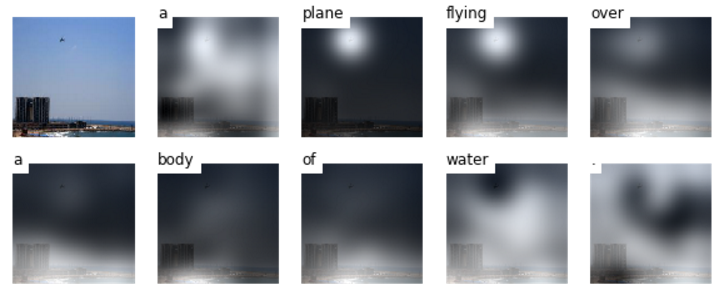
\includegraphics[width=\linewidth]{images/paper-images/show-attend.png}
\caption{Example of generation of a caption. White areas in the images visualize the attention for each of the corresponding words of the generated caption\protect\footnotemark.}
\label{fig:show-attend}
\end{figure}

\footnotetext{Image taken from: github.com/kelvinxu/arctic-captions}

Figure \ref{fig:show-attend} shows an example of caption generation with localization of attention areas for each word in the caption. Separating the salient objects in different images is especially useful when an image contains lots of them. In that case, compressing all the salient parts in a single image would result disordered and unintuitive.



\section{Explanation via Saliency Masks}

The philosophy of the approaches based on Saliency Masks consists in describing what are the parts of the record that contribute the most to the prediction of the black box. A \textit{Saliency Mask} is a subset of the record to be explained (i.e. a specific part of an image or a subset of words in a text) that causes the black box to make that specific prediction. 

In the case of saliency masks, the function to extract them strictly depends on the type of model under analysis (e.g. Convolutional Neural Network), making these approaches not model-agnostic.
\bigskip

The strategy adopted by \cite{neural-attention} consists in the generation of attention maps for a Convolutional Neural Network, which simply highlight salient regions of an image and localize various categories of objects. Such maps are generated with the help of a backpropagation scheme that the authors call \textit{Excitation Backprop}. This approach basically combines bottom-up and top-down information (in reference to the direction of data flow in a CNN) to assign each neuron the probability of being relevant to the selected prediction (i.e. a selected output unit). Then, starting from these probabilities, we can generate soft attention maps that summarize the contribution of each neuron to the prediction. We call them "soft" because they do not specify strict boundaries: rather, they are heatmaps that represent the probability distribution of the most relevant neurons.
Note that, in this setting, each neuron of a convolutional layer can be matched with a specific area of the image.
\bigskip 

In \cite{fong}, Fong et al. present a model-agnostic framework that defines saliency masks as \textit{meaningful perturbations}. The goal is to study the effect of deleting specific regions from an image to find those that are maximally informative with respect to the prediction.

The ideal solution is to find the smallest \textit{deletion mask} that, when applied, causes the prediction of the black box to drop significantly. Such mask is then presented to the user as an explanation.

One problem of this approach is that, sometimes, deletion masks can trigger artifacts. Artifacts are particular inputs that can cause Neural Networks to generate unexpected output. Usually, masks that contain artifacts look unintuitive and unnatural and this impacts heavily on the quality of the visual explanation. 
To solve this issue, the authors of \cite{fong} suggest not to focus on the specific details of the mask and apply a random jitter. Also, since artifacts masks are not good representatives of natural perturbations, they force them to have a simple and regular structure.
\bigskip

In parallel with \cite{fong}, the authors of \cite{real_time_image_saliency} developed a saliency detection method that can be performed by single forward pass (rather than interatively, like in \cite{obj-detectors}) and produces high quality and sharp masks. To address the problem of artifacts, their solutions is to \textit{crop} the image rather than masking it. The goal is to find the tightest rectangular crop that contains the entire salient region of the image.



To evaluate the quality of such explanations, they also introduce a \textit{saliency metric} defined as:

\begin{equation}\label{eqn:saliency-metric}
s(a,p) = log(\widetilde{a}) - log(p)
\end{equation}

where $a$ is the area of the cropped region (as fraction of the image size) and $p$ is the probability assigned by the black box to class $c$ (the class of the original image) when feeding it the cropped image. $\widetilde{a}$ defines the minimum threshold and is just $max(a,0.05)$. The lower this value, the more precise and sharp is the saliency region.

\begin{figure}
\centering
\begin{subfigure}[b]{.49\linewidth}
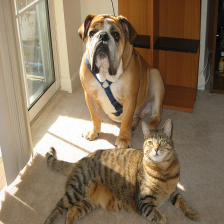
\includegraphics[width=\linewidth]{images/paper-images/grad-cam-orig.png}
\caption{Original image}
\label{subfig:grad-cam-orig}
\end{subfigure}
\begin{subfigure}[b]{.49\linewidth}
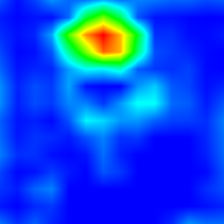
\includegraphics[width=\linewidth]{images/paper-images/grad-cam-mask.png}
\caption{Class Activation Mapping}
\label{subfig:grad-cam-mask}
\end{subfigure}
\caption{Grad-CAM: the image on the left is the original one, while the one on the right defines the Class Activation Mapping for the label \textit{boxer}\protect\footnotemark.}
\label{fig:grad-cam}
\end{figure}
\footnotetext{Image taken from: github.com/ramprs/grad-cam}

To produce the desired masks, the authors develop a \textit{masking model} that can operate in a single forward pass. The model takes the image and its class as input and outputs masks that minimize a certain objective function (of which Equation \ref{eqn:saliency-metric} is a part).\bigskip

Other techniques, such as those presented in \cite{zhou, gradcam} (CAM, Grad-CAM), incorporate neuron activations in their visual explanations. Note that, for this reason, the only family of models that can be explained is the one of Convolutional Neural Networks (for various tasks such as Image Captioning and Visual Question Answering).

These approaches use the gradients of a given target concept (i.e. the class to be explained) in the final convolutional layer to create a sort of heatmap that highlights the important regions in the image that contributed the most to the concept prediction (an example of such maps is shown in Figure \ref{fig:grad-cam}).

Convolutional features, in fact, contain visual information that would be lost if we moved to the fully-connected layers. Neurons in convolutional layers look for semantic information in the image (e.g. ears of a cat, stripes of a zebra) and Grad-CAM uses the gradient to understand the importance of each neuron (hence of each region of the image) in the prediction process.\bigskip



All the previous methods focused on defining, each with a different strategy, a \textit{pixel level} explanation identifying "unstructured" relevant areas inside images. Those areas may indeed highlight a mixture of features that, when put together, are not well defined and distinct any more. 

In contrast, the method illustrated in \cite{interpretable-convnets} aims at producing explanation at \textit{object-part level} that specify clear, distinct and highly interpretable parts of an image. The authors' approach is based on the definition of \textit{Interpretable CNNs}: the basic idea is to modify the way features are represented inside filters of convolutional layers. 

\begin{figure}
\centering
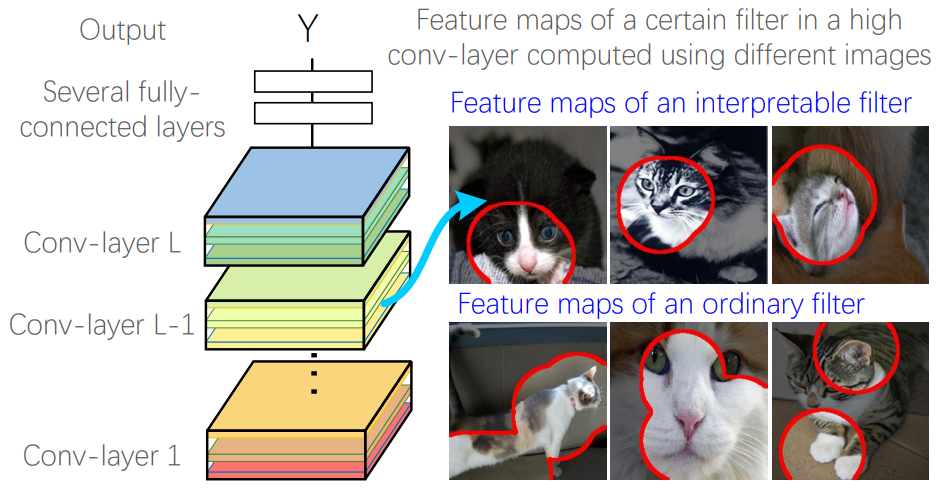
\includegraphics[width=.9\linewidth]{images/paper-images/interpretable-convnets.png}
\caption{Comparison of the features of a traditional CNN and an interpretable CNN. Filters of the first one identify different patterns at the same time (e.g. ear and legs of a kitten), while interpretable filters only highlight a single part which, in this case, is the kitten's face (image taken from \cite{interpretable-convnets}).}
\label{fig:interpretable-convnets}
\end{figure}


In traditional CNNs, as we just mentioned, filters may describe multiple patterns all at once. The advantage of an Interpretable CNN is that each of the filters in a convolutional layer is trained to match a single object part. To do that, the authors propose to define a loss function that pushes filters to the representation of an object part.
The ultimate goal is to make features interpretable, so that they can be presented to the user as an explanation.
Figure \ref{fig:interpretable-convnets} shows the differences between filters of traditional and interpretable convnets. 

\section{Alternative image data representations}

The most popular way of representing images typically makes use of a matrix of pixels (actually, a three-dimensional tensor for RGB images) with a fixed structure, in the sense that pixels are ordered and there is nothing that memorizes their spatial structure.

The authors of \cite{bag-of-pixels} propose to model images as bags of pixels (or set of vectors). If we take grayscale images as an example, such bags are collections of tuples of the form (X, Y, I) where (X, Y) are the spatial coordinates of the pixel and I the \textit{intensity} value. One advantage of this representation is that it is permutational invariant, making it suitable for variations such as morphing and translation. Taking the latter as an example we note that, in the classic matrix representation, such an operation would result highly non-linear. Translating a grayscale image by $k$ pixels, in fact, would require to multiply it by a shifting matrix raised to the power of $k$ (because we only have a basis of variation, the intensity of the pixels). 

On the other hand, in the bag of pixels representation we simply add a constant factor to the (X, Y) coordinates of each tuple inside the bag (we now have two more bases of variation). This means that, in this representation, an image can translate or morph by using a simple linear transformation. Rather than a representing a fixed concept, bags of pixels allows images to be viewed as a manifold of possible vectorized configurations.
\bigskip

Another way to represent images in classification tasks is the visual \textit{bag-of-words} (BOW), as described in works such as \cite{bag-of-keypoints, yang-visual-words, yang2-visual-words, old-visual-words, visual-word-reconstruction}. This idea is adapted from the standard BOW commonly used in information retrieval and natural language processing for text data. In that scenario, a document is represented by an histogram that counts the number of occurrences of each word appearing in the document itself. 

We can exploit the same concept for image data, but the difference is that we use images' features (regions, specific patterns etc.) instead of words. For the sake of comprehension, we can think of them as \textit{visual words}. 

In this setup, an image is then represented as a set of features, which will be used to build the "vocabulary" of visual words (typically by using a clustering algorithm) and extract the histogram representation of images. Figure \ref{fig:visual-bag} illustrates such a process on a toy example. To detect such features, one can use one of the many feature extractor algortihms (such as \cite{sift}). Histograms are then used to train a classifier or to find similar images. 


\begin{figure}
\centering
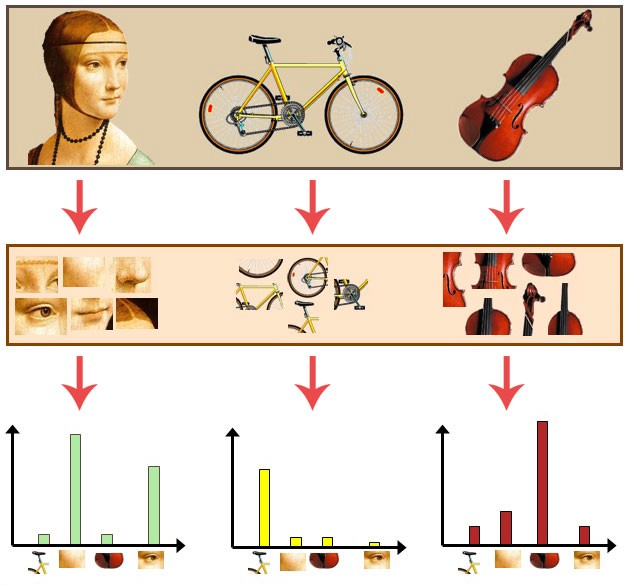
\includegraphics[width=.5\linewidth]{images/paper-images/visual-bag.jpeg}
\caption{Example showing the visual bag-of-words generation process. From each image, we extract a set of features and use them to build the visual vocabulary (shown in the X-axis of the histograms)\protect\footnotemark .}
\label{fig:visual-bag}
\end{figure}
\footnotetext{Image taken from: \\ towardsdatascience.com/bag-of-visual-words-in-a-nutshell-9ceea97ce0fb}

The traditional visual BOW approach, however, gives rise to two drawbacks. The first one has to do with the high amount of features generated for each image. We have to define a large amount of features if we want to obtain better performances, but at the same time an oversized vocabulary would slow down the prediction process (up to excessive amounts of time). The authors of \cite{visual-bag-of-words} propose a visual BOW reduction that aims at reducing the size of the features' vocabulary, using spectral clustering. 



The other problem is the fact that, when generating the visual BOW, this approach only uses low-level, purely visual features without considering the high-level semantics. This can lead to a consistent reduction of the performances in more sophisticated operations. 
We may think for example to the task of grouping together all the images that belong to a certain broad category, e.g. pictures about sports: by considering only low-level visual features, we would not be able to assign the same category to an image representing a rugby match and another depicting a swimming race. In fact, in the first one we would only obtain an histogram revealing the presence of a ball, helmets, grass and so on, while in the second we would only get water, swim goggles, swimming cap etc. Images inside the same category may look visually different, so if we just focused on details we would not be able to capture the high-level meaning.

To overcome this issue, the authors of \cite{visual-bag-of-words} propose to enrich the vocabularies with some tags previously assigned to images (i.e. their high-level semantic). They call this process \textit{visual BOW refinement}. In particular, they use a graph-based approach to define a multi-class, semi-supervised learning problem. The graph is meant to represent the semantic of the images and is built using both the low-level features and the tags.


\section{Comparison with the state of the art}

In this section we define what are the main commonalities and differences between the work presented in this thesis and those belonging to the state of the art.
As we explained at the beginning of this chapter, our goal is to explain the predictions of images made by a black box classifier. In particular, we consider predictions that always refer to one object at a time, i.e. we limit ourselves to a \textit{single-object recognition} task. 

Solutions similar to those presented in \cite{show-and-tell, show_attend_and_tell} focus instead on capturing the whole content of an image, describing in details all the objects appearing in the image itself and the relations among them. In comparison, we can refer to those tasks as \textit{scene recognition}.

Going back to single-object recognition tasks, our approach shares some properties with \cite{gradcam, neural-attention, zhou}: those methods propose the definition of maps (or masks) that highlight the most salient regions of an image with respect to a certain prediction. The final result is indeed not very different from ours: in both cases, the user can clearly distinguish what are the areas of the image that contribute the most to the prediction made by the black box. 

There is however a fundamental difference in the way these explanations are generated. In \cite{gradcam, neural-attention, zhou}, maps are created by digging into the architecture of the black box (therefore it is not a black box anymore), which must be a CNN. The idea behind those solutions is to establish the contribution of different neurons in convolutional layers to the actual prediction. After selecting the most relevant ones, the mask is generated by highlighting the corresponding features in the image. 
Being tightly coupled with the architecture of the black box makes these approaches unusable in many situations.

What we propose is then a \textit{model-agnostic} explanation system that completely abstracts from the type of black box used. In producing our explanations we indeed use the model as a pure black box: we just need its predictions, not caring about the way they are made.
To do so, we plan to build linear, interpretable models that approximate the behavior of the black box in the neighborhood of the image to be explained.

In \cite{fong}, the authors follow the exact same principle: to build explanations, in fact, they just focus on the images themselves, trying to identify informative regions by applying what they call \textit{meaningful perturbations}. The type of black box is again irrelevant, because the goal consists in studying how the model reacts to certain perturbations.

Finally, as far as regards the way images are represented, our approach differs from those that propose to include semantic aspects in the representation of images \cite{bag-of-keypoints, yang-visual-words, yang2-visual-words, old-visual-words, visual-word-reconstruction, bag-of-pixels, visual-bag-of-words}. Since we plan to highlight, cut and replace contiguous patches of pixels, the most natural choice is to use matrices of RGB values.

\chapter{Background: LIME}\label{chapt:background}
In this chapter we explain in detail the strategy adopted by \textit{LIME} (\textit{Local Interpretable Model-agnostic Explanations})\cite{lime}, which is the starting point of this thesis' work. The main topic we cover are \textit{explanations}: we will see that, sometimes, it is necessary to explain the predictions of a black box classifier so that people using it can also trust it. The kinds of explanations we may think of are various (depending on the type of data under analysis), such as textual and visual feedback. In this work we are focused on explaining predictions on images: LIME provides explanations consisting of highlighted areas inside the images, representing patterns that contribute the most to the final outcome of the black box. 

In standard scenarios, machine learning models are often evaluated using accuracy, precision and other metrics based just on the outcome of the classifier. 
The idea behind LIME is to exploit explanations as an additional evaluation parameter: if a classifier has low accuracy but is able to generate intuitive explanations (whether the prediction is right or not), then the users will trust it and people who developed it can understand better what is going on inside the opaque structure of the model.

To evaluate the explanations themselves, the authors of \cite{lime} define the concept of \textit{interpretability}. Explanations need to be simple enough to be understood by the majority of people, even those ones who are not experts. For instance, when explaining the prediction of a decision tree, it is recommended not to include more than 4-5 statements in the explanations (in other words, the tree's depth should not exceed a certain value). 
Or, in case of linear models, it might be better to keep the explanation readable, limiting as much as possible the number of features having non-zero weights.

\section{Explaining the predictions}

In our terminology, explaining a prediction corresponds to provide the user with feedback that can help him to understand clearly what are the relationships between the given input data and the output data. In the specific case of image predictions, an explanation is just a set of areas in the picture the black box looks at to take its decision. 

\begin{figure}
\begin{center}

 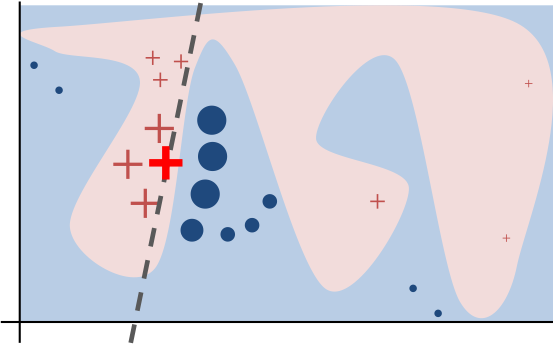
\includegraphics[scale=1]{images/easy_model.png}
 \end{center} 
\caption[]{The black box's complex decision boundary (blue and light red areas) is locally approximated by a linear model (dashed line). The red bold cross is the instance to be explained and the other crosses and blue dots represent the instances in the neighborhood. Their size is proportional to their weight: we can see that the noise points that are far from the instance are almost ignored.\footnotemark}
\label{fig:decision_bound}
\end{figure}

\footnotetext{Image taken from:\\
https://raw.githubusercontent.com/marcotcr/lime/master/doc/images/lime.png }

One important characteristic of a good explainer is the ability to explain the predictions of any classifier, without making any assumptions on its internal structure. These methods are therefore \textbf{model-agnostic} and the models, as we already pointed out, should only be seen as plain black boxes. Many of the most performant models in the literature have extremely complex structures (\textit{Random Forests} and \textit{Convolutional Neural Networks}, just to name a few), so when it comes to practice one should not limit himself by choosing simple (and possibly inaccurate) models.

We also need to point out that, every time we say "explanation", we mean "local explanation" (for more details, see section \ref{chapt:related-work}). The decision function of the black box may have a boundary that is too complex to be interpretable (Figure \ref{fig:decision_bound}). What LIME tries to explain are just the single outcomes, taken one at a time. Giving a general, complete and exhaustive description of the entire model is a hard, challenging task and it still remains an unsolved problem in the state of the art.


\section{The need for interpretability and fidelity}

Every single time we ask LIME for an explanation, it needs to build a simple, interpretable model that mimics sufficiently well the black box in the vicinity of the image that is being analyzed. 
\textit{Interpretability} is fundamental because explanations need to be crystal clear to anyone and \textit{fidelity} ensures that the interpretable model captures the local behavior of the black box.

To ensure interpretability, LIME builds ad-hoc \textit{Interpretable Data Representations} (IDR). In the case of image classification, we can think of "shattering" the picture into a set of areas (regardless of their shape) made of contiguous pixels. An IDR can therefore be defined as an array of bits telling whether or not the single areas are present.

Note that IDRs \textit{do not} necessarily correspond to the features used by the model in the prediction process. 
Such features, indeed, may be arbitrarily complex structures that are not suitable for being shown to the end user. Convolutional Neural Networks, for instance, use convolutional \textit{feature maps} as internal representations of images in the hidden layers.

Fidelity, instead, is obtained by choosing the model that best approximates the black box in the vicinity of the image. Defining the opposite of the fidelity as the \textit{locality loss} and the opposite of interpretability as \textit{complexity}, LIME's goal can be reconducted to a minimization problem defined by the following equation:

\begin{eqnarray}
model = \arg\min_{g \in G} \;\; locality\_loss(g) + complexity(g)
\label{eqn:bestmodel}
\end{eqnarray}

where $G$ is the class of interpretable models (in the case of LIME, $G$ is the family of linear regression models). More precisely, $complexity(g)$ defines how understandable the model $g$ and its explanations are. For linear models, we can think of this measure as the number of non-zero weights in the final regressor: if we have many of them, we cannot distinguish clearly the relevant features in the explanation.

As for $locality\_loss(g)$, it can be seen as the degree of similarity between $g$ and the black box. From the models having the lowest value of $complexity$, one should choose the one that better approximates the behavior of the black box in the vicinity of the instance to be explained (even if it is not the simplest one). The best model is then the solution of Equation \ref{eqn:bestmodel}, which minimizes both the $complexity$ and $locality\_loss$.

\section{Generation of the neighborhood}

As we have already mentioned, LIME looks for an interpretable model that is able to replicate the local behavior of the function represented by the black box. Among all the possible models, it clearly wants to pick the best one in terms of fidelity. Ideally, LIME could simply choose the model $g \in G$ that minimizes the right-hand side of Equation \ref{eqn:bestmodel}. 

While it might be simple to compute the term $complexity(g)$ just by looking at the structure of the model (depth of decision tree, weights of a regressor etc.), there is no way to determine exactly the term $locality\_loss(g)$, because it obviously depends on the black box's function: in order to build a model-agnostic explainer, indeed, no assumptions should be made on the type of black box used. 

What can be done, instead, is approximating the local behavior of the black box by seeing how it reacts to variations in the input images. To do that, a certain number of samples is drawn from the domain of the IDRs. In the case of LIME, such domain includes binary vectors

\[
	w \in \{0,1\}^k
\]

where $k$ denotes the number of features in the image (contiguous patches of pixels) and each term of $w$ indicates the fact that the corresponding feature is included (in case the value is equal to 1) or not (value is equal to 0). Each one of such terms is called an \textit{Interpretable Component}. 
In the rest of this work, the words \textit{feature, patch, area, piece} will be used interchangeably to denote the exact same concept.

Once the number of images in the vicinity is fixed, LIME starts generating an equal number of vectors $w$ uniformly at random, assigning them a weight that is proportional to their distance from the original image. By doing this, LIME gives less importance to the noisy images (that are too far away to be considered neighbors) and focuses just on the samples that are close to the original picture.
We need to point out that, in this domain of IDRs, the original image is represented by a vector having all its entries set to 1 (intuitively, the original image maintains all of its patches).

\begin{figure}
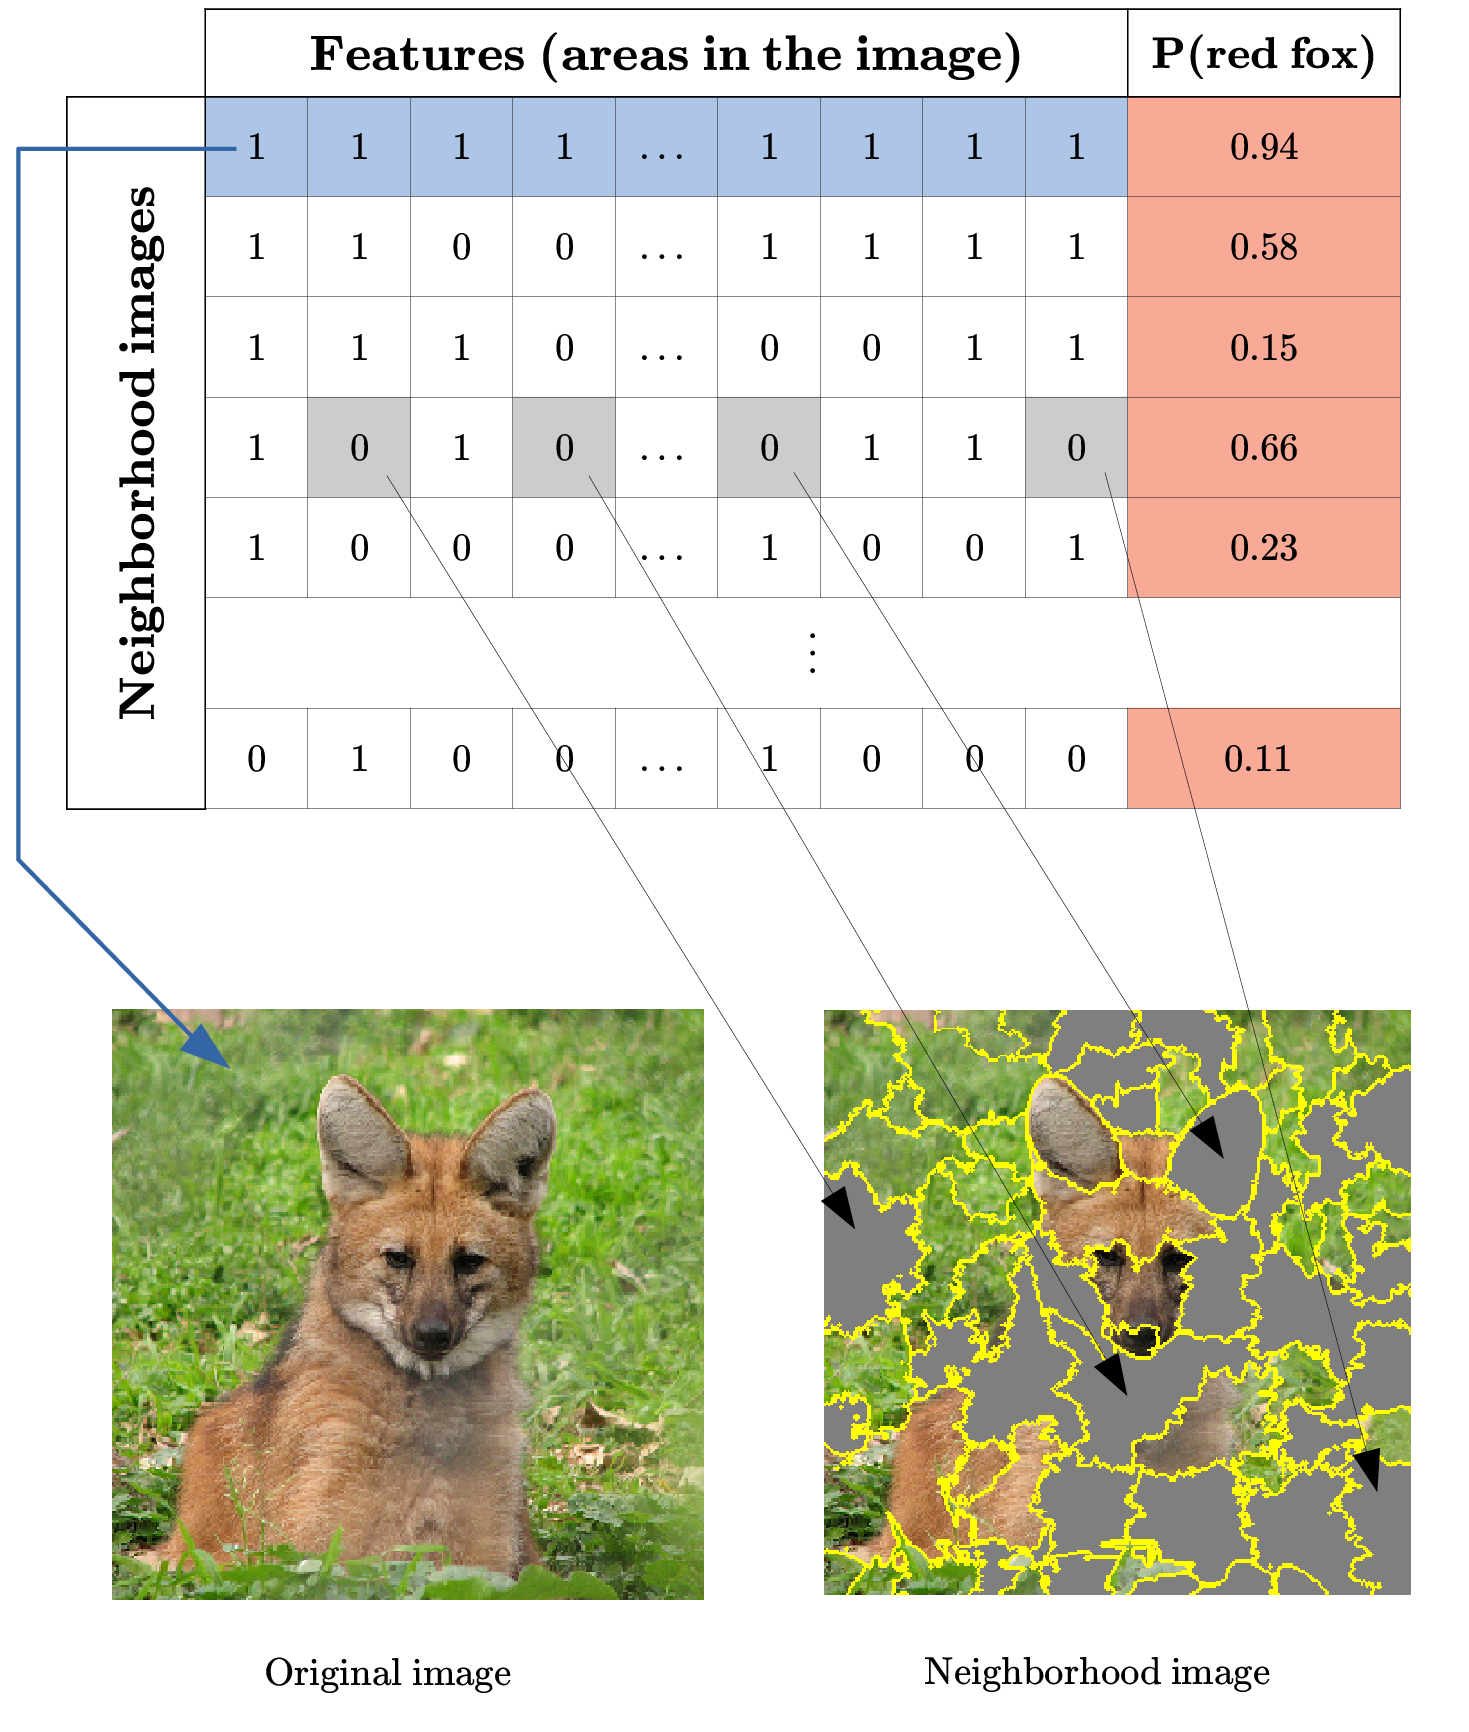
\includegraphics[width=\textwidth]{images/neighborhood_gen.png} 
\caption{The neighborhood generation process adopted by LIME. \textit{"red fox"} is the prediction we want to explain. The first row of the matrix (highlighted in blue) is the IDR of the original image, and the remaining ones represent images in the neighborhood.}
\label{fig:neighborhood_generation}
\end{figure}

Figure \ref{fig:neighborhood_generation} gives an idea of what neighborhood images look like. Each row of the table represents a vector of \textit{Interpretable Components} and there is a column for each one of the areas in which the image has been split. We find the original image in the first row.

To generate the image corresponding to the i-th row, LIME starts from the original picture and, every time it finds an entry set to 0, it \textbf{turns off} the corresponding area. In the example shown in Figure \ref{fig:neighborhood_generation}, turning off simply means replacing the pixels with plain gray areas, but of course different strategies can be adopted (like replacing the patches with the average of the pixels or picking pieces from other images).
In the neighborhood image depicted in Figure \ref{fig:neighborhood_generation}, we highlighted in yellow all the areas (features) the image has been split into. We can see that they are all contiguous patches of pixels and, in this case, they also have an irregular shape. In particular, they were obtained using \textit{quickshift}\cite{quickshift}, which is an algorithm based on an approximation of kernelized mean-shift\cite{meanshift}.

Keeping the label of the real image as a reference, LIME applies the black box model to each of the images that have been generated, obtaining an array 

\[
	preds \in  [0, 1]^{n}\subset \mathbb{R}^{n}
\]

of prediction probabilities (the one highlighted in red in Figure \ref{fig:neighborhood_generation}), where $n$ is the total number of samples in the neighborhood. Each value represents the probability that the black box still assigns the original label to a certain neighborhood image after all the perturbations are applied.
This allows to observe how the predictions change when changing the input, giving a good approximation of the local behavior of the black box model.

Once the $preds$ array is obtained, it is used to learn a regression model where the loss function is the linear least squares function and the regularization is given by the l2-norm (also known as Tikhonov regularization). In the model, the input variables are the IDR arrays and the targets are the corresponding probabilities inside $preds$.
 
The model that best approximates the black box is the one that minimizes the loss function and the learned weights (as many as the number of entries of each IDR) define a measure of importance among the features. In particular:

\begin{itemize}
\item if the weight is \textbf{positive}, it means that the associated area of the image contributes positively to the prediction of the black box;
\item if the weight is \textbf{negative}, then the corresponding feature goes against the prediction.
\end{itemize}

Now we have all the ingredients to define precisely what is an explanation (from the point of view of LIME). Given an image $x$ and a prediction $p$ that needs to be explained, an explanation 
\[
	\mathcal{E}(x,p)
\]

is just a set of tuples of the form $(f_{i},w_{i})$ where $f_{i}$ is the i-th feature of the image (i.e. a patch, contiguous area of pixels) and $w_{i}$ is the weight associated to that feature by the regression model. To obtain a sort of visual feedback from this raw data, LIME only considers the best $n$ tuples (after ordering them by their weights, in descending order) and highlight the corresponding features in the image. Intuitively, those will be the areas where the black box looks when making such a prediction. Examples of explanations can be found in the next chapter, where we explain our approach more in detail.

\section{Gaining insights about wrong predictions}

\begin{figure}
\centering
\begin{subfigure}[b]{.49\linewidth}
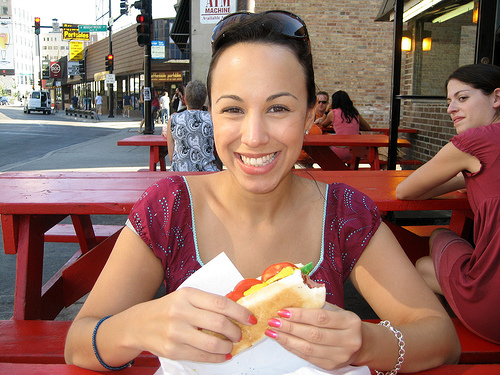
\includegraphics[width=\linewidth]{images/insight-original.JPEG}
\caption{Original image.}
\label{subfig:insight_orig}
\end{subfigure}
\begin{subfigure}[b]{.49\linewidth}
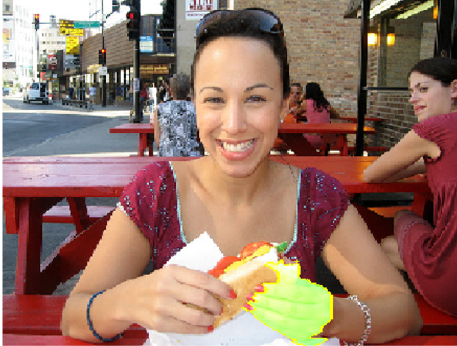
\includegraphics[width=\linewidth]{images/insight-resized.png}
\caption{Explanation for \emph{candle}.}
\label{subfig:insight_exp}
\end{subfigure}
\caption{Example of explanation of a wrong prediction: the original image was meant to represent a \emph{hotdog} (image on the \textbf{left}), while the predicted label is \emph{candle} (image on the \textbf{right}).}
\label{fig:insight}
\end{figure}

Trusting the model is a key factor when it comes to prediction tasks. One of the main concerns, of course, is the model's ability to output the correct predictions given certain input data. The minimization of the discrepancy between the real classes and the predicted ones is the goal of the so-called \textit{learning} phase. However, there are cases in which this is not enough and we need to trust the model's predictions. Rather than treating it as an oracle, one might need to know what is the reasoning behind the process and what are the relationships between the input and the output. 
An example is the usage of machine learning models in medical diagnosis\cite{healthcare}: if the model claims that a patient has a certain disease, doctors may need to know what are the factors that cause it in order to trust the prediction.

Note that these requirements must apply to both correct and wrong predictions: in the first case, we want to make sure that the prediction is reasonable (and not based on luck or randomness), while in the second one we want to understand the causes of an error (so that it can be fixed). 
The strategy adopted by LIME meets all those requirements as it shows the user what are the exact areas of the image that contribute to the prediction. It is then the user's responsibility to judge the correctness of the prediction.


Figure \ref{fig:insight} shows an example of wrong prediction. The image on the left (Figure \ref{subfig:insight_orig}) portrays a girl holding a hot dog in her hands. The correct label for this image is indeed \textit{hotdog}. When feeding that image to the black box, the outcome is completely wrong (\textit{candle}). Apparently, there are no candles in the picture, so we cannot even suspect what went wrong during the prediction process. However, when we use LIME to get an explanation for the label \textit{candle}, we immediately understand what led the model astray: the fingers of the girl's left hand were recognized as candles (due to their shape and the presence of the nail polish). The corresponding area is indeed the only part of the image that has been highlighted.

\chapter{Proposed approach}\label{chapt:approach}
The goal of this work is to extend LIME by experimenting an alternative way to generate the neighborhood of a given image when trying to come up with an explanation for the class predicted by the black box. 

To get started, we will use a different segmentation technique that is based on a grid-like approach to measure the impact of the features' shapes on the quality of the explanation (we will give different definitions of "quality" of an explanation later on). Various sizes of the grid will be used so that the analysis will result as exhaustive as possible. 

Another parameter that we would like to tune is the way features of the input image are replaced (or \textbf{turned off}) when generating images in its vicinity. The original version of LIME provides two alternative ways:

\begin{enumerate}
\item replacing all the pixels in the feature with a plain color (e.g. gray, black or white). In the following, we will use the gray color and call this variant \textbf{LIME gray};
\item replacing the pixels' values with the mean value of all the pixels inside the specific region. We can think of this technique as a sort of undersampling of the image. We will denote this version as \textbf{LIME color}.
\end{enumerate}

The main idea of our work, instead, is to replace the patches by picking "pieces" of different images, drawn from a \textit{test set}.

For this reason we propose to modify the feature generation process towards a grid-style one. The original strategy exploits a segmentation algorithm that defines meaningful regions of an image. These regions, however, strongly depend on the contours of the objects appearing in the image itself. In the image-based neighborhood generation process, if we cut out pieces from other images by using those shapes, we would not be able to capture any interesting pattern. Also, we would run the risk of putting together pieces of different patterns.

The way we choose images, of course, leads to different versions of the explainer. Later on we will see what is the difference between picking completely random images and choosing specific ones using clustering algorithms (depending on the image we are explaining). 

In the next sections, we will illustrate an example of application of all the versions on the same image (Figure \ref{fig:tricycle}).

\begin{figure}
\begin{center}
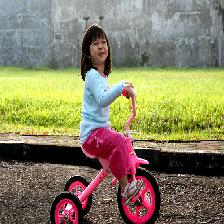
\includegraphics[scale=1]{images/tricycle.JPEG} 
\caption{Sample image to be explained by all the versions of LIME. The correct prediction for it is \emph{tricycle}.}
\label{fig:tricycle}
\end{center}
\end{figure}

\section{LIME}

The first version we propose is the original one, in which features are extracted via a segmentation algorithm. In particular, we present two variants of this version that use different colors to replace the features of the images.

For the first variant we choose the color gray to turn off the features (we will refer to it as LIME gray). As a consequence, images in the neighborhood will have gray patches here and there (see Figure \ref{fig:lime_neigh}). The features are the result of the quickshift segmentation algorithm and their shape tends to adapt to the edges of all the objects appearing in the picture.

\begin{figure}
\begin{center}
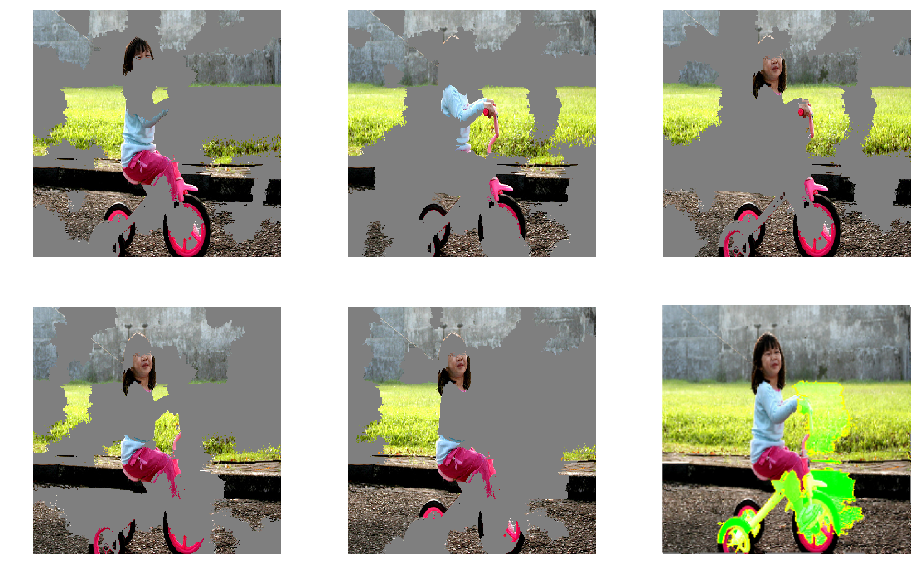
\includegraphics[width = .85\textwidth]{images/lime_neighborhood.png} 
\caption{Neighborhood images generated by LIME gray (images from 1 to 5, counting from left to right and from top to bottom) and explanation for the label \textit{tricycle} (\textbf{bottom-right}).}
\label{fig:lime_neigh}
\end{center}
\end{figure}

An explanation is composed by the image with some highlighted patches. These patches indicate areas that positively contribute to the prediction \emph{tricycle}. In Figure \ref{fig:lime_neigh} we see that most of the highlighted spots include the tricycle itself, while there are some parts of the explanation that cover apparently useless details (like the grass and the road). 
One important thing to notice is that, since we are explaining the label \emph{tricycle}, the little girl is not included in the explanation.

%\begin{figure}
%\begin{center}
%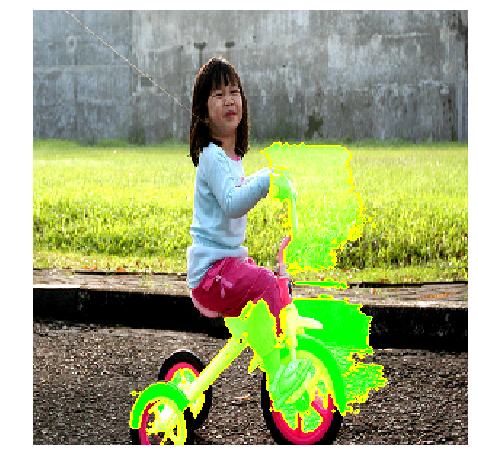
\includegraphics[width = .6\textwidth]{images/lime_explanation.png} 
%\caption{Explanation given by LIME gray for the label \emph{tricycle}.}
%\label{fig:lime_exp}
%\end{center}
%\end{figure}

\bigskip

The next variant we present is again the original one, but this time we replace the turned off features with the average value of all the pixels inside them (we will refer to this variant as LIME color). Here the result is a little bit different from the previous version: as we can see in Figure \ref{fig:limecolor_neigh}, it looks like the images are somehow undersampled in correspondence of the features that were turned off. The result is that the predominant color in the patches replaces all the other pixels.

\begin{figure}
\begin{center}
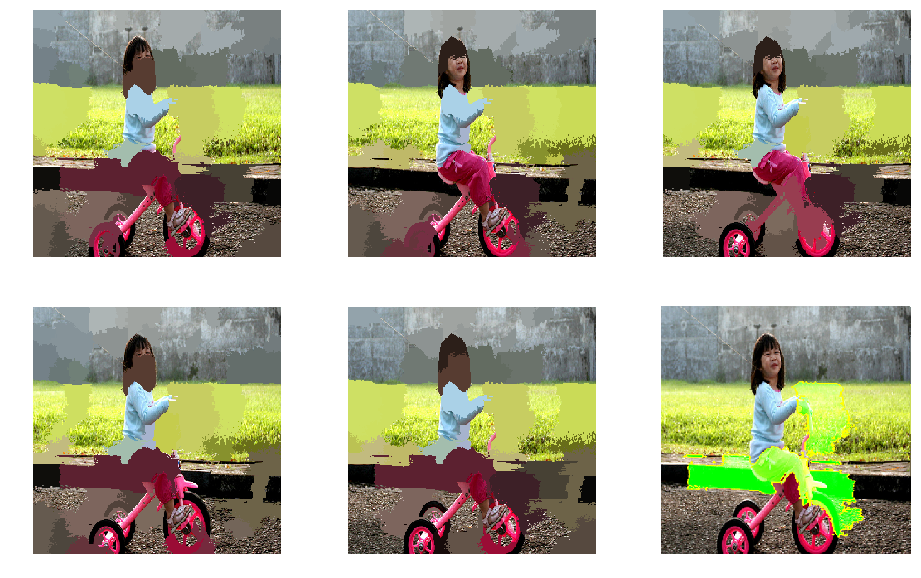
\includegraphics[width = .85\textwidth]{images/limecolor_neighborhood.png} 
\caption{Neighborhood images generated by LIME color (images from 1 to 5, counting from left to right and from top to bottom) and explanation for the label \textit{tricycle} (\textbf{bottom-right}).}
\label{fig:limecolor_neigh}
\end{center}
\end{figure}

%\begin{figure}
%\begin{center}
%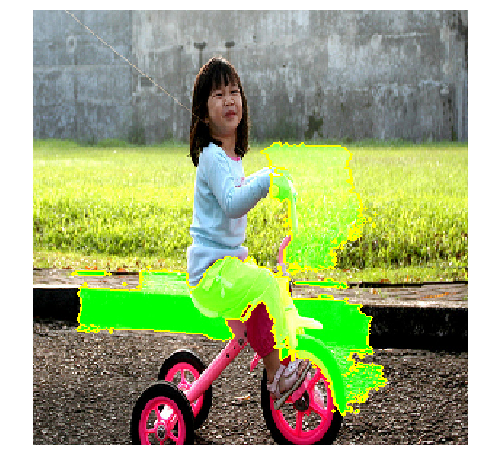
\includegraphics[width = .6\textwidth]{images/limecolor_explanation.png} 
%\caption{Explanation given by LIME color for the label \emph{tricycle}.}
%\label{fig:limecolor_exp}
%\end{center}
%\end{figure}

If we take a look at the explanation given by LIME color in Figure \ref{fig:limecolor_neigh}, we notice that it is pretty different from the one given by LIME gray. This time, the tricycle is not sufficiently covered by the highlighted areas: the only relevant part that is included are the handlebars, while the crossbar and the wheels are completely excluded. 
In addition to that, the irrelevant parts increased (road, sidewalk and grass). 



\section{LIME$\#$}

The next version we present is LIME\#. The feature replacement strategy is the same as LIME, but in this case the patches have a squared shape (as if the image were split into a regular grid). We propose again two different variants, based on the way we replace features. For the first one, we use the gray color to replace turned off features and refer to it as LIME\# gray. 

The size of the grid has to be specified by the user, but in the example in Figure \ref{fig:limesharp_neigh} it is fixed to 8x8. This time it is evident that features do not have shapes that adapt to the image subject (they are not the result of a segmentation algorithm anymore). They are just squares at fixed positions and the result is that there are some "oversized" gray pixels here and there.

\begin{figure}
\begin{center}
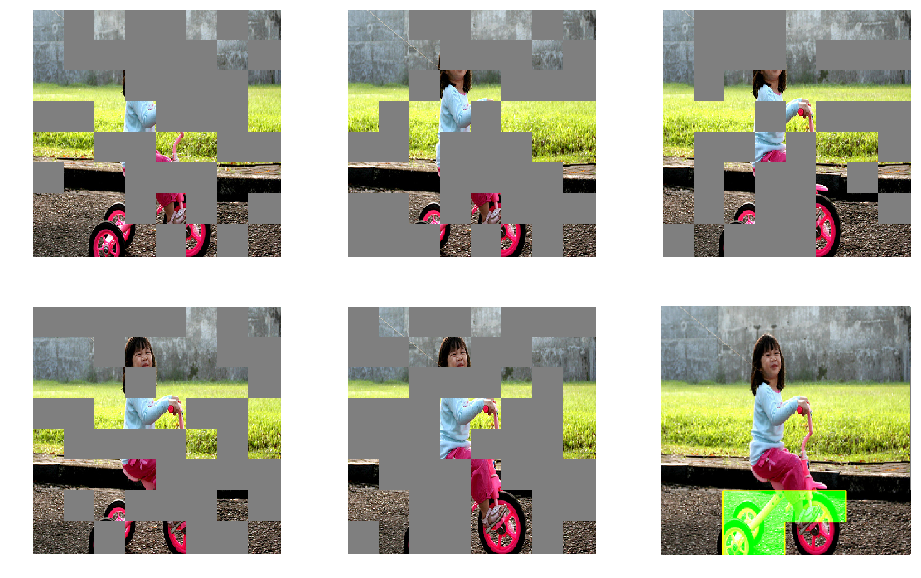
\includegraphics[width=.85\textwidth]{images/limesharp_neighborhood.png} 
\caption{Neighborhood images generated by LIME\# gray (images from 1 to 5, counting from left to right and from top to bottom) and explanation for the label \textit{tricycle} (\textbf{bottom-right}).}
\label{fig:limesharp_neigh}
\end{center}
\end{figure}

The explanation illustrated in Figure \ref{fig:limesharp_neigh} is simpler than the previous ones and has now a much cleaner aspect. The motivation for the prediction \textit{tricycle} is also very intuitive as the highlighted areas include the vast majority of the tricycle. Even though the front wheel has not been entirely captured, there are no irrelevant parts in the explanation.

%\begin{figure}
%\begin{center}
%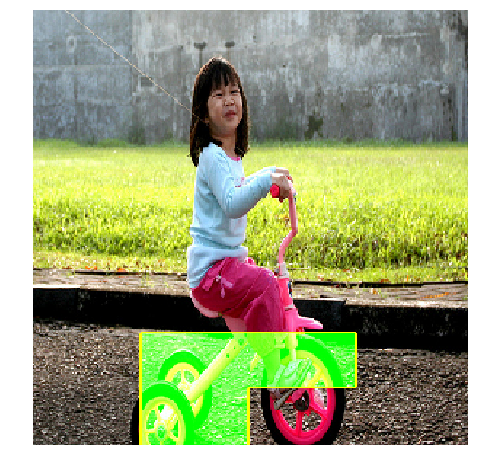
\includegraphics[width=.6\textwidth]{images/limesharp_explanation.png} 
%\caption{Explanation given by LIME\# gray for the label \emph{tricycle}.}
%\label{fig:limesharp_exp}
%\end{center}
%\end{figure}

\bigskip

Next we present LIME\# color, which is the variant of LIME\# that uses the average value of the pixels to replace turned off features. Even in this case, the grid size has been fixed to 8x8 so that the explanation can be compared to the one of LIME\# gray variant. 

By looking at Figure \ref{fig:limesharpcolor_neigh}, images in the neighborhood are partially filled with low-resolution, oversized pixels.

\begin{figure}
\begin{center}
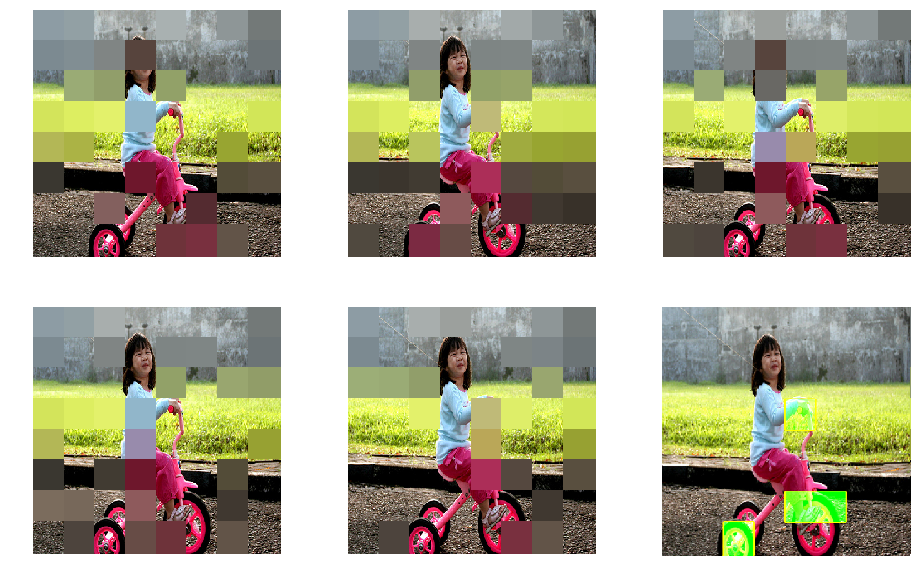
\includegraphics[width=.85\textwidth]{images/limesharpcolor_neighborhood.png} 
\caption{Neighborhood images generated by LIME\# color (images from 1 to 5, counting from left to right and from top to bottom) and explanation for the label \textit{tricycle} (\textbf{bottom-right}).}
\label{fig:limesharpcolor_neigh}
\end{center}
\end{figure}

The explanation in Figure \ref{fig:limesharpcolor_neigh} is once again cleaner than the approaches based on quickshift segmentation and does not include irrelevant aspects of the picture. Highlighted areas are exclusively parts of the tricycle (wheels and handlebars), even though they are not completely covered.

%\begin{figure}
%\begin{center}
%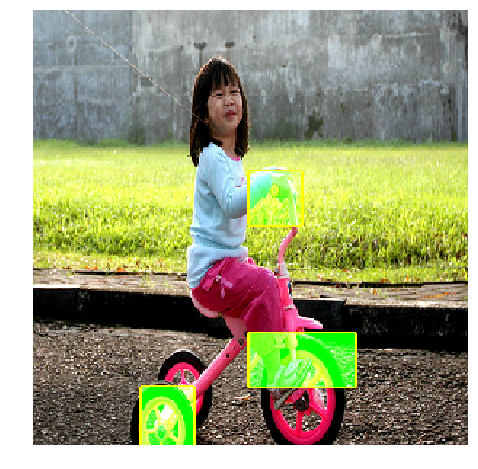
\includegraphics[width=.6\textwidth]{images/limesharpcolor_explanation.png} 
%\caption{Explanation given by LIME\# color for the label \emph{tricycle}.}
%\label{fig:limesharpcolor_exp}
%\end{center}
%\end{figure}

\section{Image-based neighborhood approaches}

This section presents the two approaches that we conveniently classify as \textit{image-based neighborhood} approaches. With respect to the already presented approaches, these ones differ in a single aspect: the neighborhood generation. In fact, images in the neighborhood are not generated by replacing areas of the original image with plain colors anymore. Rather, those patches are now filled with the corresponding patches taken from images belonging to a predefined set of images, which we will call \textit{image pool} from now on.

As we will see in the next two paragraphs, different ways of defining such image pool lead to different versions of the explainer. In particular, we will build one pool composed of random images and another one including images that are similar to the one to be explained.

\begin{figure}
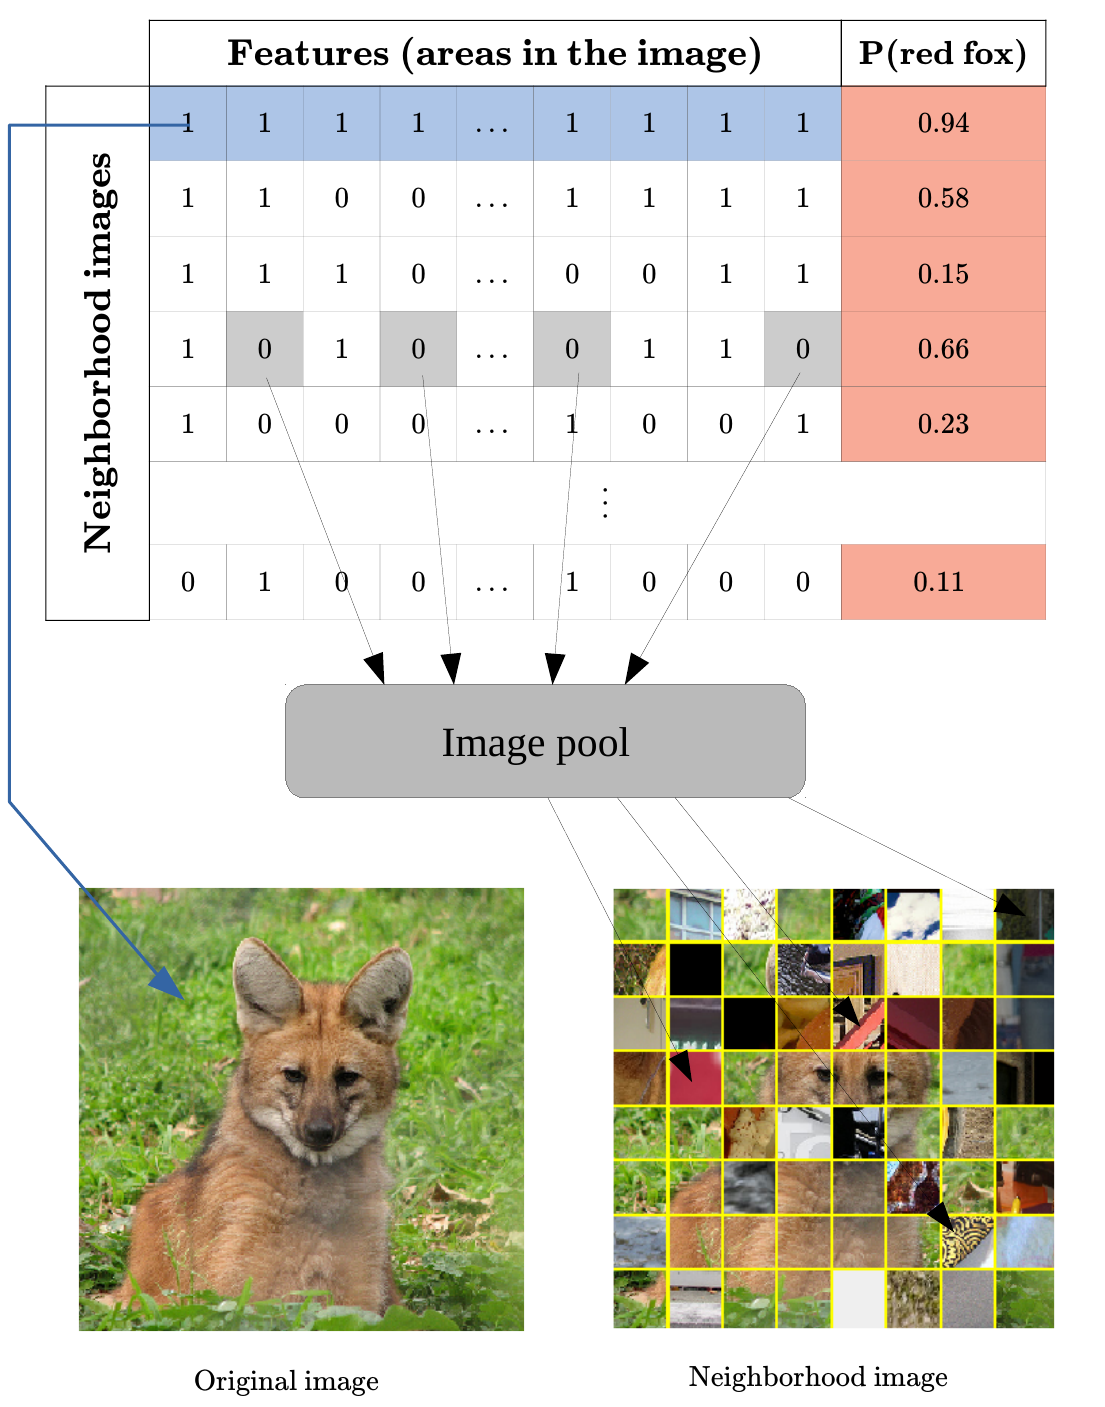
\includegraphics[width=\textwidth]{images/image-based_neigh.png} 
\caption{The neighborhood generation process adopted by image-based neighborhood approaches (LIME\#R and LIME\#C). \textit{"red fox"} is the prediction we want to explain.}
\label{fig:img-based_neigh}
\end{figure}

\subsection{LIME$\#$R}

\textit{LIME\#R} is the first of the two explainers belonging to the category of image-based neighborhood approaches. The "R" in the method name stands for \textit{Random} and it indicates how the images from the test set are drawn.

In this variant, we have that
\begin{equation}
image\,pool = I
\label{eqn:image_pool}
\end{equation}

where \textit{I} is any set of images arbitrarily chosen by the user. No specific selection criterion needs to be used when building this set.

Our proposed approach for the neighborhood generation process is described in Figure \ref{fig:img-based_neigh}. In particular, when we encounter a 0 entry in the IDR array (a single row in the matrix), we go through the following operations:

\begin{enumerate}
\item choose an image at random from the image pool;
\item cut off the part corresponding to the feature being replaced in the original image;
\item use the part of image obtained from 2) to replace the feature in the original image.
\end{enumerate}

At the end of this process, images in the neighborhood look like the one shown in Figure \ref{fig:img-based_neigh} (bottom-right). Even in this case, the shape of the features is squared (denoted by the "\#" character in the explainer's name).

Figure \ref{fig:limesharpR_neigh} gives an idea of the composition of the images in the neighborhood. Pieces of possibly unrelated images are scattered throughout the picture, but we can still detect some details of the original image.

\begin{figure}
\begin{center}
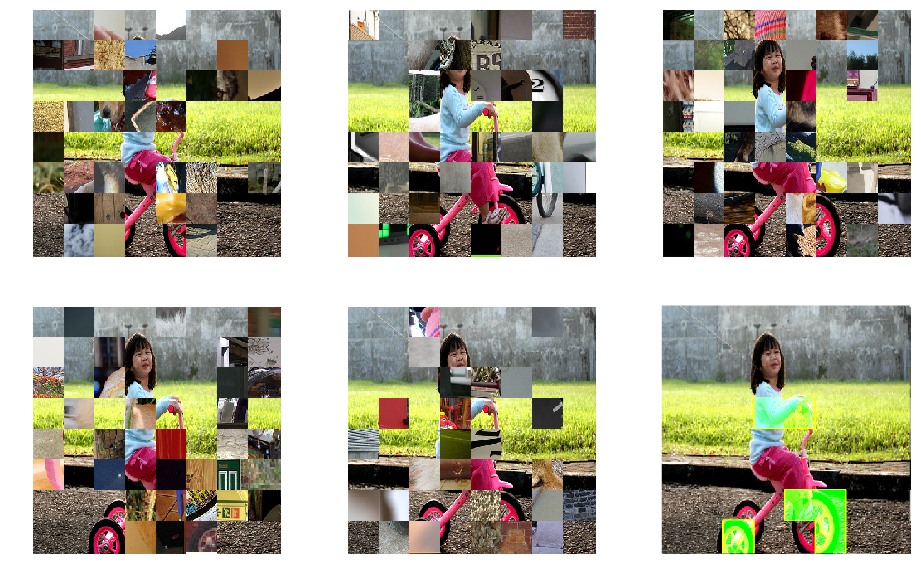
\includegraphics[width=.85\textwidth]{images/limesharpR_neighborhood.png} 
\caption{Neighborhood images generated by LIME\#R (images from 1 to 5, counting from left to right and from top to bottom) and explanation for the label \textit{tricycle} (\textbf{bottom-right}).}
\label{fig:limesharpR_neigh}
\end{center}
\end{figure}

%\begin{figure}
%\begin{center}
%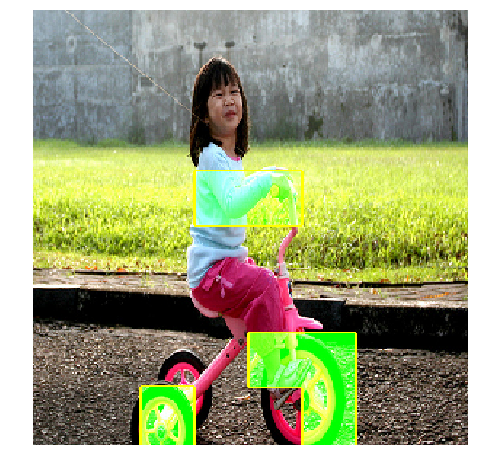
\includegraphics[width=.6\textwidth]{images/limesharpR_explanation.png} 
%\caption{Explanation given by LIME\#R for the label \emph{tricycle}.}
%\label{fig:limesharpR_exp}
%\end{center}
%\end{figure}

In Figure \ref{fig:limesharpR_neigh} we can also look at the result of the explanation: the most relevant areas for the prediction comprehend once again the wheels of the tricycle, as well as the arms of the little girl holding the handlebars.


\subsection{LIME$\#$C}

The second explainer belonging to this category is \textit{LIME\#C}. The "C" in the method name stands for \textit{Clustering} and it means that a specific clustering algorithm is used when defining the image pool.

In particular, we define the image pool for this version of LIME as 
\begin{equation}\label{eqn:limesharpC_pool}
image\,pool = \{\,i \in I\, |\, cluster(i) = cluster(original)\, \land i \neq original \,\}
\end{equation}

\noindent
where 

\begin{itemize}
\item $original \in I$ is the image to be explained;
\item $cluster:\, I \rightarrow Integer$ is the function associated to the used clustering algorithm that assigns an integer label to each image in I.
\end{itemize}

We see that \textit{image pool} only contains images that, according to the clustering algorithm, belong to the same cluster as \textit{original}. The idea behind this approach is to measure the impact of choosing similar images to construct the neighborhood instead of completely random ones.

As we previously did for \textit{LIME\#R}, we now explain in detail the neighborhood generation process. First of all, we build the image pool by applying clustering to the images in the set \textit{I}. Note that this task is only performed once (and not for each image in the neighborhood).
Then, for each 0 entry in each IDR array, we apply the same operations as before (i.e. draw an image from the pool, cut off the specific part and replace it in the original image).

\begin{figure}
\begin{center}
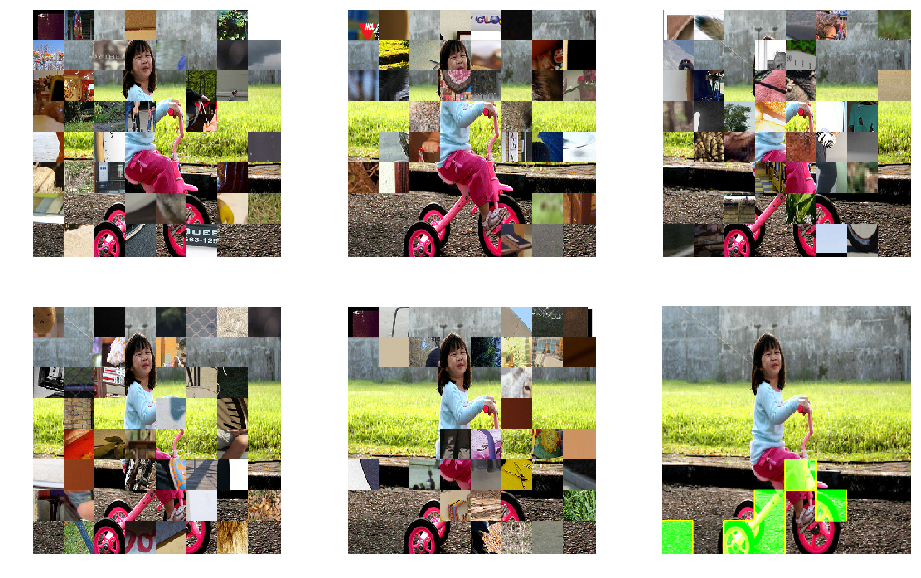
\includegraphics[width=.85\textwidth]{images/limesharpC_neighborhood.png} 
\caption{Neighborhood images generated by LIME\#C (images from 1 to 5, counting from left to right and from top to bottom) and explanation for the label \textit{tricycle} (\textbf{bottom-right}).}
\label{fig:limesharpC_neigh}
\end{center}
\end{figure}

\begin{figure}
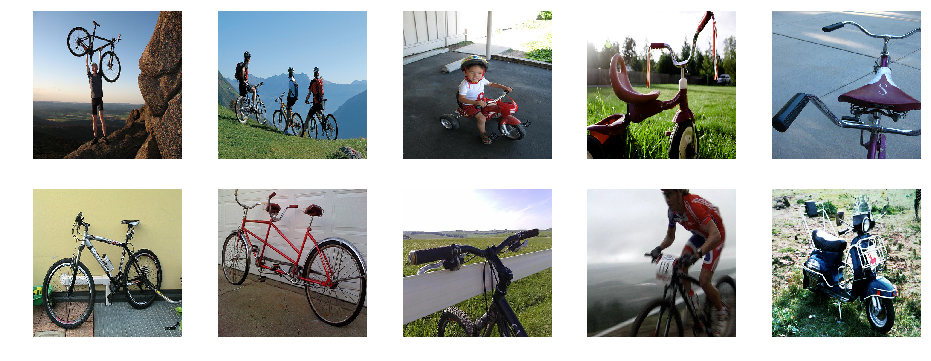
\includegraphics[width=\textwidth]{images/limesharpC_same_clus.png} 
\caption{A small sample of the images belonging to the same cluster as the image in Figure \ref{fig:tricycle}.}
\label{fig:limesharpC_same_clus}
\end{figure}

In Figure \ref{fig:limesharpC_neigh} we see that neighborhood images still contain pieces of other images, but this time we note some interesting details such as wheels of other vehicles. The point of using clustering in this scenario is exactly to group together images that are visually similar and see whether this technique has a positive or negative impact on the results.

Figure \ref{fig:limesharpC_same_clus} shows a subset of the images that belong to the same cluster as the image to be explained (the one in Figure \ref{fig:tricycle}). All of them represent bicycles, tricycles and motor scooters: in fact, the cluster seems to group together images containing the same visual details (i.e. vehicles having both wheels and handlebars).

%\begin{figure}
%\begin{center}
%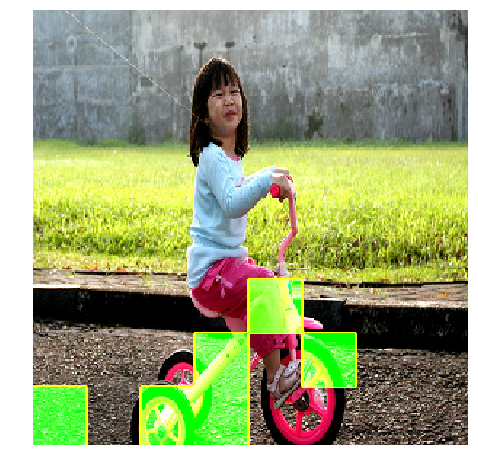
\includegraphics[width=.6\textwidth]{images/limesharpC_explanation.png} 
%\caption{Explanation given by LIME\#C for the label \emph{tricycle}.}
%\label{fig:limesharpC_exp}
%\end{center}
%\end{figure}

Finally, Figure \ref{fig:limesharpC_neigh} shows also the explanation for the label \textit{tricycle} given by \textit{LIME\#C}: some parts of the tricycle are clearly highlighted (crossbar and wheels), while others not (handlebars). In addition to that, we also spot a noisy feature (the leftmost at the bottom) highlighting the road.


%%%%%% BEGIN %%%%%%%% moved from section 5
\subsubsection{Definition of \textit{Clustering Purity}}

\begin{table}[]
\centering
\def\arraystretch{1.3}
\begin{tabular}{|l|l|l|}
\hline
\textbf{Cluster} & \textbf{Most frequent class} & \textbf{Frequency} \\\hline
Cluster 1 & analog\_clock & $23/50$ \\\hline
Cluster 2 & digital\_clock & $18/42$ \\\hline
Cluster 3 & white\_wolf & $14/45$ \\\hline
Cluster 4 & toyshop & $20/68$\\\hline
\end{tabular}
\caption{Toy example that shows how to proceed in the computation of the \textit{Clustering Purity}.}
\label{tab:cluster_purity_example}
\end{table}

In the evaluation of the cluster results we do not use the standard measures (e.g. \textit{Sum of Squared Errors} for K-means) because our idea is based on the analysis of the contents of the single clusters to look at the distribution of the images and on finding the frequency of the most frequent class in each cluster. In order to capture this idea of clustering compactness, we propose to use a measure called \textit{Clustering Purity}. 

Suppose our clustering algorithm finished its execution and found $n$ clusters: to compute the \textit{Clustering Purity}, we pick each cluster one by one and extract the most frequent class along with its frequency. Once all the values are collected, we compute the average, median and standard deviation.



Now let us try to compute the \textit{Clustering Purity} in the small example in Table \ref{tab:cluster_purity_example}. In the first column we find the clusters resulting from the execution of the clustering algorithm (with $n=4$), while in the second one we find the most frequent class in each cluster. Using the values under the column \textbf{Frequency}, we obtain that $average=0.37$, $median=0.37$ and $std=0.0719$.


\subsubsection{Clustering algorithm}



\begin{figure}
\centering
\begin{subfigure}[b]{.49\linewidth}
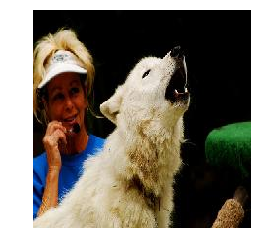
\includegraphics[width=\linewidth]{images/undersamp-orig.png}
\caption{Original image, before the undersampling process.}
\label{subfig:undersamp-orig}
\end{subfigure}
\begin{subfigure}[b]{.465\linewidth}

\includegraphics[width=\linewidth]{images/undersamp-und.png}
\caption{Undersampled image. New size is 8x8 pixels.}
\label{subfig:undersamp-und}
\end{subfigure}
\caption{Representation of the effect of the undersampling process. The image on the left (Figure \ref{subfig:undersamp-orig}) is the original image, and the one on the right (Figure \ref{subfig:undersamp-und}) is the result of the application of an undersampling process with $grid\_size = 8$.}
\label{fig:undersamp-example}
\end{figure}

To compute clustering on image data, instead of rearranging all the single pixels of the image in a monodimensional array, we apply a process of undersampling that depends on the size of the grid (the one that defines the size of the features). In other words, if we choose $grid\_size = n$ during the neighborhood generation process, then the clustering will be performed on images that have been undersampled to $nxn$ pixels.

In order to clarify how this process works, consider the following example. Suppose we choose a random image and that $grid\_size=8$: the image is then divided in $8x8 = 64$ squared regions, each having a certain number of pixels inside. Now each region is replaced by a single pixel, whose RGB values are just the average of all the RGB values of the pixels inside the region. The resulting undersampled image has then a dimension of $8x8$ pixels. Before passing this image to the clustering algorithm, it is flattened into a monodimensional array having dimension $8x8x3$ (3 is because we have 3 color channels: Red, Green and Blue).
\bigskip

We propose two variants of LIME\#C, one using the clustering algorithm \textit{K-means} and one the \textit{Spectral Clustering}.

K-means \cite{k-means} is a centroid-based algorithm. As a description of a cluster, this algorithm measures the position of its center and the spread of the cluster itself in the space (intuitively, this describes clusters as spherical shapes).
K-means is a partitional clustering approach where each cluster is associated with a centroid, i.e. a representative point that summarizes the characteristics of all the other points in the same cluster. 

K-means has one fixed parameter, K, that specifies the number of clusters we want to find. The basic idea is shown in Algorithm \ref{alg:kmeans}. Regarding the definition of the initial centroids, we could simply choose random points. Note, however, that this choice determines the quality of the result, so we may want to try different initializations and pick the one that leads to the best results. 
Also, closeness between points and centroids can be estimated by using different measures (e.g. Euclidean distance, Cosine similarity etc.).

\LinesNumbered
\RestyleAlgo{algoruled}


\begin{algorithm}
\KwIn{Number of clusters K, data to be clustered D}
\KwOut{A set of K clusters}
\Repeat{centroids don't change}{
Build K clusters by assigning all points of D to the closest centroid\;
Recompute centroids of each cluster\;
}
\caption{K-means clustering algorithm.}
\label{alg:kmeans}
\end{algorithm}

The main disadvantage of this algorithm is that it only works well when clusters have a spherical or globular shape. K-means has problems also when clusters are not all of the same size and/or they have heterogeneous densities. On top of that, the presence of even few outliers can cause a noticeable difference in the computation of centroids: at each iteration, in fact, centroids tend to adapt to the distribution of points inside their clusters (even the noisy ones that are far away from the others).

\bigskip

The second one, Spectral Clustering \cite{on-spectral-clus,spectral_clustering, spectral-tutorial}, is an algorithm that performs dimensionality reduction exploiting the \textit{spectrum} (hence the name \textit{Spectral}) of the similarity matrix of the data. The general approach consists in using a standard clustering algorithm (that can be K-means itself) on special instances, which are some relevant eigenvalues of the Laplacian of the similarity matrix. The Laplacian matrix is a particular representation of a graph $G$ and is defined as 

\begin{equation}
L = D - A
\end{equation}


where $D$ is the degree matrix of $G$ (a diagonal matrix that contains the degree of each node) and $A$ is its adjacency matrix.

This algorithm is particularly useful when the structure of the clusters is highly irregular and cannot be described by a convex, spherical shape.

Such similarity matrix can be either given as an input (precomputed) or computed on-the-fly using a function that outputs the pairwise distances among all the instances in the data set (e.g. \textit{Radial Basis Function}). 

%%%%%%% END %%%%%%%%%% moved from section 5


\begin{table}[]
\def\arraystretch{1.6}
\begin{tabularx}{\textwidth}{|c|X|}
\hline
\textbf{LIME version} & \textbf{Description} \\ \hline
LIME gray & Original version of LIME. Turned off features are replaced with a gray color.\\ \hline
LIME color & Original version of LIME. Turned off features are replaced with the mean value of all the pixels inside them.\\ \hline
LIME\# gray  & It is the original version of LIME in which the segmentation function has been changed to a grid-style fashion. Turned off features are replaced with a gray color. Note that the "\#" indicates the grid-style segmentation.\\ \hline
LIME\# color & Same as above. This time, turned off features are replaced with the mean value of all the pixels inside them.                                                                                                                                                         \\ \hline
LIME\#R      & Features are replaced with pieces of images from a test set, drawn at random. R stands for \textit{Random}.                                                                                                                                                                                                \\ \hline
LIME\#C      & As above, we pick pieces of images from a test set. However, this time the test set is made of images belonging to the same cluster as the original image. C stands for \textit{Clustering}.\\ \hline

\end{tabularx}
\caption{Summary of the different versions of LIME.}
\label{tab:lime_versions}
\end{table}
\bigskip

%%%%%%%%%%%%%%%%%%%%%%%%
To summarize, Table \ref{tab:lime_versions} lists the unique characteristics of all the versions of LIME we have presented so far.


\chapter{Experiments}\label{chapt:experiments}

In this chapter we test all the different versions of LIME described in the previous section. We will present the data set used for the evaluation of the explanations, then we will define different measures of interest and, in particular, we will specify which kind of images were chosen for the task (chosen classes, their distribution etc.). 

The main points we will address during our experiments are the following:

\begin{itemize}
\item how well do the explanations approximate the exact area of the image containing the real label?
\item is the model able to distinguish between instances belonging to similar classes?
\item what is the impact of changing the neighborhood generation process?
\item is it useful to generate ad-hoc neighborhood images, using visually similar images when replacing features?
\item what is the ideal size of the images' features?
\item what is the ideal number of features an explanation should highlight to be as intuitive as possible?
\end{itemize}

We will also compare the results of different clustering algorithms (used for \textit{LIME\#C}) and the impact of choosing different grid sizes to define the dimensions of each single feature in the images.
The experiments\footnote{Source code can be found at: github.com/leqo-c/Tesi} were performed on Ubuntu 16.04.5 64 bit, 504 GB RAM, 3.6 GHz Intel Xeon CPU E5-2698 v4.

\section{Black box model}

The black box model that we have used in our experiments is \textbf{Inception v3} (introduced in \cite{inception-v3} along with \textbf{Inception v2}), which is an improvement of the \textbf{Inception v1} network first described in \cite{inception-v1}. Before explaining the basic idea (and the possible improvements) behind the architecture of Inception v1, we will now make some considerations about the contents of images. 

As we know, Convolutional Neural Networks operate on salient parts of the image (better known as \textit{features}) rather than on the single pixels. For instance, if we consider a picture of a bicycle, we may think of a feature as one of its wheels. If features were always of the same dimension, we could simply adapt the size of a filter in the convolutional layer to fit exactly  those features across different images. However, those parts might obviously vary in size in each image, so there is no such thing as a "correct" size to be used for the convolution operation. 

A na\"ive solution would be to stack convolution layers of different sizes on top of each other, but potential drawbacks would immediately arise: not only it would be computationally expensive, but also excessively deep networks are likely to overfit the data. 

The solution of Inception v1 still considers the usage of convolutions of different sizes, but the key factor is that they are applied on the exact same layer (rather than be spread in different, consecutive ones). In other words, instead of going deeper, the network goes wider. The outputs of such operations are then concatenated before being sent to the next layer. 

\begin{figure}
\centering
\begin{subfigure}[b]{.49\linewidth}
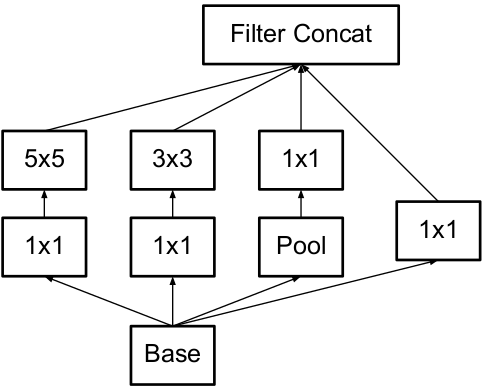
\includegraphics[width=.95\linewidth]{images/paper-images/inception-v1.png}
\caption{Original Inception v1 module, containing expensive 5x5 convolutions (described in \cite{inception-v1}).}
\label{subfig:inception-v1}
\end{subfigure}
\begin{subfigure}[b]{.49\linewidth}
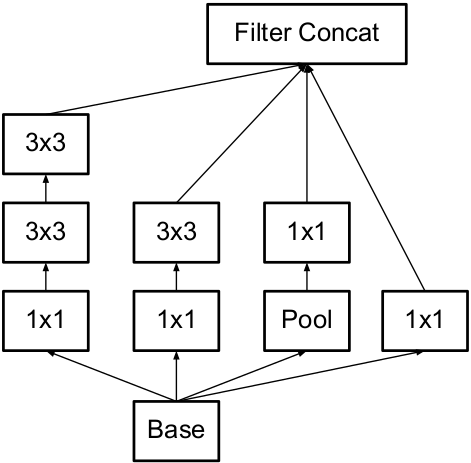
\includegraphics[width=.95\linewidth]{images/paper-images/inception-v3.png}
\caption{Inception v3 module: 5x5 convolutions are replaced by two 3x3 convolutions (described in \cite{inception-v3}).}
\label{subfig:inception-v3}
\end{subfigure}
\caption{Comparison between Inception v1 and Inception v3 modules. Both images were taken from \cite{inception-v3}.}
\label{fig:inception-versions}
\end{figure}
\bigskip

The usage of large convolutions, however, often leads to the so-called \textit{representational bottleneck}. Reducing drastically the dimension of the images, in fact, inevitably causes a loss of information. On top of that, large convolutions are computationally expensive to apply. The solution adopted by Inception v3 overcomes these drawbacks by factorizing the expensive 5x5 convolutions to two consecutive 3x3 convolutions. This operation leads to a boost in performances because 5x5 convolutions are \textbf{2.78} slower than their 3x3 versions. The process is shown in Figure \ref{fig:inception-versions}. When describing Inception v3, we are also summarizing the improvements made by Inception v2.

Another type of factorization involves a general $nxn$ convolution: the authors of \cite{inception-v3} found that factorizing a $nxn$ convolution into a pair of $1xn$ and $nx1$ convolutions made the process 33\% cheaper. 

In addition, as we mentioned before when talking about the representational bottleneck, they expanded these operations to make the module wider (rather than deeper). 
Finally, Inception v3 introduced other optimizations such as \textit{Root Mean Square Propagation} (RMSProp), factorized 7x7 convolutions and Label Smoothing (a regularization component added to the loss formula, prevents overfitting).

\section{Dataset} \label{sect:dataset_used}

All the images used in our experiments were taken from the \textit{ImageNet Large Scale Visual Recognition Challenge} 2012 (ILSVRC2012)\cite{ilsvrc}. This data set represents a benchmark in object category classification and detection on hundreds of object categories and millions of images. 

The images were chosen from the validation set, which includes 50000 images belonging to 1000 different classes. They are of any kind, ranging from animals, buildings, tools and other objects that are part of everyday life. Each class is equally frequent, and for each one we have exactly 50 images representing it.

For the purpose of our experiments, we decided to sample a subset of 1000 images belonging to 20 different classes, keeping them equally distributed (50 images per class). Table \ref{tab:chosen_classes} shows the single classes, grouped by their category. We have chosen to group together similar objects to test the model's ability to distinguish between small particulars. We also wanted to check whether the explanations were sufficiently clear or not and to know how the model makes a distinction between, for example, a \textit{toyshop} and a \textit{bookshop}.

\begin{table}[]
\def\arraystretch{1.2}
\begin{tabularx}{\textwidth}{|XXXXp{2.5cm}|}
\hline
\multicolumn{5}{|c|}{\textbf{Category}} \\ \hline

\textbf{Food} & 
\textbf{Animals} & 
\textbf{Clocks} & 
\textbf{Shops} & 
\textbf{Vehicles} \\ \hline

cheeseburger & timber\_wolf & analog\_clock & tobacco\_shop & motor\_scooter \\
hotdog & white\_wolf & digital\_clock & barbershop & mountain\_bike \\
 & red\_wolf & digital\_watch & bookshop & unicycle \\
 & coyote & wall\_clock & toyshop & tricycle \\
 & dingo &  &  & bicycle-built-for-two \\ \hline
\end{tabularx}
\caption{Chosen classes (from ILSVRC2012 data set) for the construction of the data set used in the experiments. For each of the 20 classes, we picked all the 50 corresponding images (1000 in total).}
\label{tab:chosen_classes}
\end{table}

\subsection{Definition of \textit{reference area}}

After running any version of LIME to explain the prediction of a black box for a certain image, what we get is just a set of areas in the picture that (ideally) should identify specific areas of the image that are mainly responsible for that prediction. However, there is no such thing as an information attached to the image that defines the correct boundaries of what we need to explain. To solve this problem, we need to isolate the parts of the image that contain meaningful information (in the sense of the explanation) and test how well the explanations given by LIME can cover them. In the following, we will refer to these parts as \textit{reference area}. 

To do so, starting from the data set we have just selected (see Table \ref{tab:chosen_classes}), we have cut out the parts that best represent the object specified in the image's label, filling all the remaining parts with a plain white color. We have applied this process to each of the 1000 images of the data set: the result is a new, enriched data set that can be used as a reference when evaluating explanations. A sample image from such data set is shown in Figure \ref{fig:ground_truth}.

Note that the reference area should be the one that justifies the prediction of the black box, even when it is wrong (i.e. the output of the black box is different from the actual label of the image). This is because our goal is to explain the (possibly wrong) outcomes of the black box, not the real labels themselves. In fact, when the prediction is different from the real class, we want to know what caused the error. 

To make an example, let us consider again the two images in Figure \ref{fig:insight}: the actual label of the image on the left is \textit{hotdog}, while the predicted one is candle. When defining the reference area, one should not cut out the hot dog that the girl is holding, but rather something that resembles a candle(s). In this case, the fingers of her left hand.


\begin{figure}
\centering
\begin{subfigure}[b]{.49\linewidth}
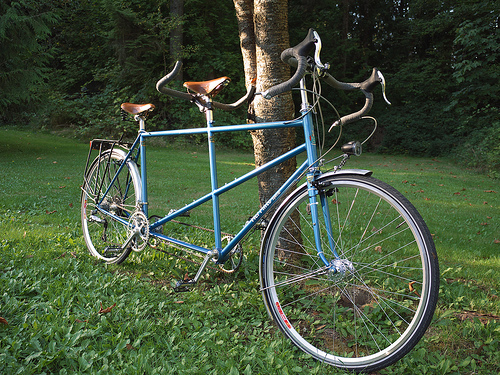
\includegraphics[width=\linewidth]{images/original.JPEG}
\caption{Original image. The label to be explained is \textit{bicycle-built-for-two}.}
\label{subfig:gt_orig}
\end{subfigure}
\begin{subfigure}[b]{.49\linewidth}
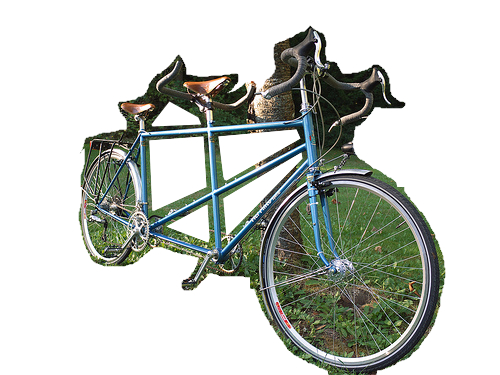
\includegraphics[width=\linewidth]{images/ground_truth.jpg}
\caption{Image defining the reference area for \textit{bicycle-built-for-two}.}
\label{subfig:gt_groundtruth}
\end{subfigure}
\caption{Example of cropped image that defines the reference area for \textit{bicycle-built-for-two}: the more an explanation covers it, the better. The image on the left (Figure \ref{subfig:gt_orig}) is the original one, while the one on the right (Figure \ref{subfig:gt_groundtruth}) highlights the silhouette of the bicycle.}
\label{fig:ground_truth}
\end{figure}

\section{Evaluation}

In order to compare the different versions of LIME, we needed to define a measure of \textit{quality} among the explanations. Intuitively, we wanted to measure the ability of the explanations to cover the reference area. The more they cover it, the more they can be trusted. Of course, the simplest explanation we can think of (the one that covers the entire image) meets these requirements, but it is not useful at all. Any explanation that highlights parts outside the reference area should be penalized in some way.

\begin{figure}
\begin{center}
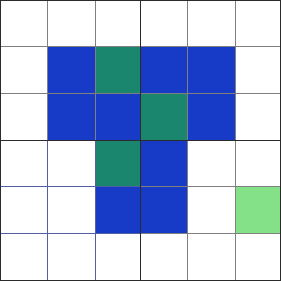
\includegraphics[width=.5\textwidth]{images/measures.png} 
\caption{Toy example that explains the computation of the precision, recall and F-measure measures. For simplicity, we suppose each square is a pixel and each green area is a feature. The T-shaped blue part is the reference area, while the green areas are the highlighted features of the explanation.}
\label{fig:measures}
\end{center}
\end{figure}

Our experimental setup took into account three different measures: \textit{precision}, \textit{recall} and \textit{F-measure}. The precision of an explanation tells us what is the percentage of highlighted areas that fall into the reference area. If all those areas (regardless of the number) are inside the reference area, the precision is 1. If all of them are outside the reference area, precision is 0. In particular, precision is defined as 

\begin{equation}
precision =
\frac
     {\#\,highlighted\,areas\,inside\,reference\,area}
     {\#\,highlighted\,areas}      
     \label{eqn:precision}
\end{equation}

This is coherent with the standard definition of precision (which is $\frac{TP}{TP+FP}$) because the highlighted areas in the reference area are actually \textit{True Positives} and the ones outside it are \textit{False Positives}.

The next measure is recall, which can be considered the ability of the explanation to cover the reference area. Specifically, it measures the percentage of pixels in the reference area covered by the explanation. It is defined as

\begin{equation}
recall = 
\frac
	{\#\,highlighted\,pixels\,in\,reference\,area}
	{\#\,pixels\,in\,reference\,area}
     \label{eqn:recall}
\end{equation}

Even in this case, we find a correspondence between this formula and the standard definition of recall (that is $\frac{TP}{TP+FN}$): each highlighted pixel in the reference area is indeed a \textit{True Positive}, while the remaining ones (still inside the reference area) are erroneously uncovered (\textit{False Negatives}).

The final measure we use is the F-measure, that considers both the precision and the recall in its computations. It is defined as 

\begin{equation}
F\textnormal{-}measure = 
	2 \cdot \frac
	    {precision \cdot recall}
        {precision + recall} 
\label{eqn:fmeasure}
\end{equation}

Figure \ref{fig:measures} helps us computing the above mentioned measures in a toy example. First of all we note that the reference area (blue part) is made of 12 pixels, while the explanation highlights 4 different areas (of 1 pixel each). 

To compute the precision of such explanation, we exploit the formula in Equation \ref{eqn:precision}: in total, the explanation highlights 4 areas, 3 of which are inside the reference area. The value we are looking for is then $\frac{3}{4} = 0.75$. This means that 3 areas are actually \textit{True Positives}. 

To compute the recall, we refer instead to Equation	\ref{eqn:recall}. Remember that in the example of Figure 	\ref{fig:measures} each square is a pixel. The reference area has 12 pixels in total, with only 3 of them being highlighted. The recall of the explanation is then $\frac{3}{12} = \frac{1}{4} = 0.25$. Intuitively, this amounts to say that the explanation covers only the 25\% of the entire reference area.

Finally, we compute the F-measure using Equation \ref{eqn:fmeasure} and the two previously computed measures. We have

\begin{align*}
F\textnormal{-}measure 
&= 2 \cdot \frac{0.75 \cdot 0.25}{0.75 + 0.25} = 0.375
\end{align*}

\section{Results}

In this section we will analyze the results of the different versions of LIME (in terms of precision, recall and F-measure) and make a comparison among them. In defining the size of the grid representing images' features, we will use the following values: 4x4, 8x8, 16x16, 32x32, 64x64.

For each of the newly defined versions, we will also study the pros and cons with respect to the original version of LIME. We will also focus on the differences between LIME\#R and LIME\#C to measure the effects of using clustering during the neighborhood generation process. For reasons of readability, plots of performances for increasing values of $grid\_size$ have been moved to the Appendix.

\subsection{LIME\# gray}

First, we evaluated the performances of the explainer as the number of highlighted areas increases, comparing different sizes of the grid with the base version LIME gray. Figure \ref{subfig:limesharp_gray_vs_sf} shows the values of precision, recall and F-measure for fixed numbers of highlighted areas. 


\begin{figure}
\centering

\makebox[\textwidth][c]{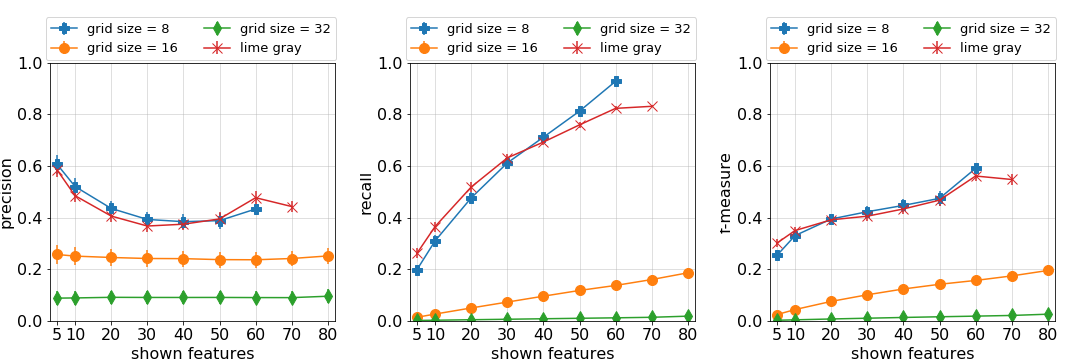
\includegraphics[width=1.1\linewidth]{images/figs/lime-sharp-gray-all.png}}

\hspace{-4mm} 
\caption{LIME\# gray: Precision, recall and F-measure for increasing values of the parameter $shown\_features$.}
\label{subfig:limesharp_gray_vs_sf}
\end{figure}



The precision of the explanation reaches a maximum of about 0.6 (Figure \ref{subfig:limesharp_gray_vs_sf}) when using either LIME\# gray with $grid\_size = 8$ or LIME gray (highlighting 5 features in both cases). For $shown\_features \leq 50$, we see that LIME\# gray outperforms LIME gray. In addition, we note a progressive decrease until $shown\_features$ reaches the value 60, where the precision rises again. 
Higher values of $grid\_size$, 16 and 32 in particular, have a negative impact on the precision, which tends to stabilize around low values (about 0.25 and 0.1 respectively).

Even for the recall, LIME\# gray with $grid\_size=8$ and lime gray behave differently with respect to the versions that use higher values for the grid size. In the first case, recall reaches about 0.8 (even more when $grid\_size = 8$), while in the second case it is always below 0.2.

Finally, the F-measure behaves similarly to the recall, except for the fact that now the maximum value is about 0.6 (when $shown\_features = 60$, as before). What is evident from these plots is that the performances drop significantly when $grid\_size$ gets higher and higher. This is because, in the explanations, small features cannot cover sufficiently well the reference area and, most importantly, they are not sufficiently big to capture the relevant patterns in the images.
\bigskip

Performances for all the possible values of $grid\_size$ are shown in the Appendix (Figure \ref{fig:limesharp_gray_vs_gs}). We immediately see that when $grid\_size \geq 32$ we get poor results (for all the measures). Again, this is because higher grid sizes lead to the definition of very small areas that, rather than patterns, resemble more the single pixels.
Also, we note that the more features we highlight the better. However, this is not true for the precision: in fact, Figure \ref{subfig:limesharp_gray_prec_vs_gs} shows that we reach a precision of above 0.5 when using a grid of 8x8 and highlighting just 10 features.

\subsection{LIME\# color}

The next version we will focus on is LIME\# color. Figure \ref{subfig:limesharp_color_vs_sf} shows its performances for different values of $shown\_features$ and $grid_size$, also making a comparison with LIME color.

For $grid\_size = 16$ and $grid\_size = 32$ we reach a precision of about 0.25 and 0.1, respectively. For $grid\_size = 8$, instead, we see that LIME\# color always outperforms LIME color, reaching a precision of more than 0.6 in correspondence of $shown\_features = 5$.

\begin{figure}
\centering
\makebox[\textwidth][c]{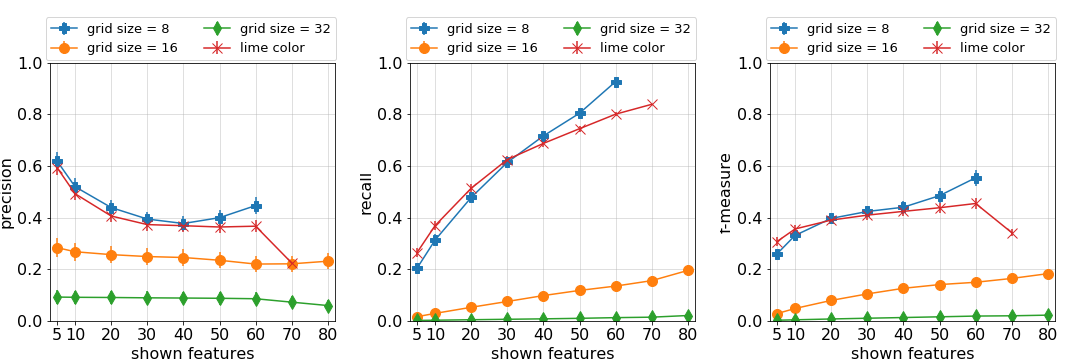
\includegraphics[width=1.1\linewidth]{images/figs/lime-sharp-color-all.png}}
\caption{LIME\# color: Precision, recall and F-measure for increasing values of the parameter $shown\_features$.}
\label{subfig:limesharp_color_vs_sf}
\end{figure}

For the recall, we have a behavior that is similar to the already mentioned LIME\# gray. LIME\# color performs better than LIME color when $shown\_features \geq 30$ and worse when $shown\_features < 30$. Once again, grid sizes higher than 8 cannot even surpass the 0.2 threshold, both for recall and F-measure. 
Finally, we note that the F-measure reaches a maximum of about 0.55 when $grid\_size = 8$ and $shown\_features = 60$. 
\bigskip

From the point of view of the grid size, Figure \ref{fig:limesharp_color_vs_gs} in the Appendix shows that when $grid\_size \geq 32$, performances are extremely poor (for all the measures). 
In accordance to what we have already stated for LIME\# gray, we note that a low number of highlighted areas improve the precision, while a high number improves recall and F-measure (Figure \ref{fig:limesharp_color_vs_gs}). 

\subsection{LIME\#R}\label{sect:limesharpR_expe}

Using Equation \ref{eqn:image_pool}, we set $image\,pool = I$ where $I$ is the set of all the sampled images used for the experiments (see Section \ref{sect:dataset_used} for more details). 

Figure \ref{subfig:limesharp_R_vs_sf} summarizes the performances of LIME\#R in terms of precision, recall and F-measure. 
By keeping LIME gray as the main element of comparison between the two versions, let us see whether the introduction of pieces of other images is significant or not (with respect to using a plain gray color). In other words, let us see whether LIME\#R performs better or worse than LIME\# gray.

In the case of precision, when $grid\_size = 8$ the results are slightly worse than those of LIME\# gray, except when $shown\_features = 60$. In that case precision rises above 0.5, surpassing LIME gray. For $grid\_size \geq 16$, the differences are so small that are not worth mentioning.

\begin{figure}
\centering
\makebox[\textwidth][c]{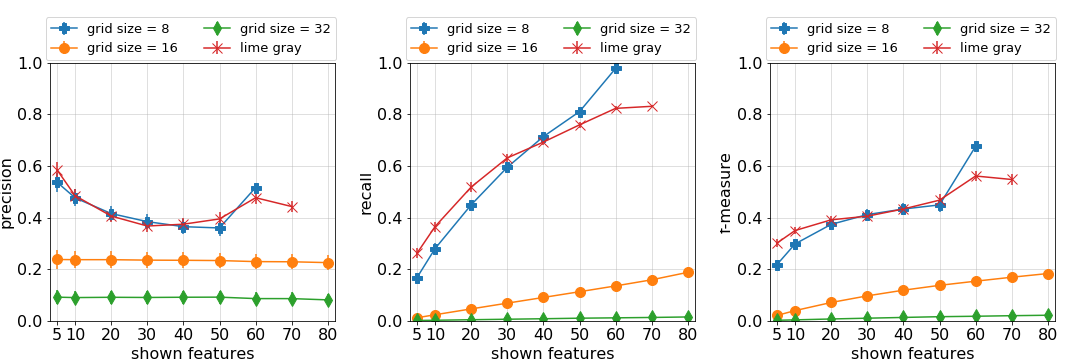
\includegraphics[width=1.1\linewidth]{images/figs/lime-sharp-R-all.png}}
\caption{LIME\#R: Precision, recall and F-measure for increasing values of the parameter $shown\_features$.}
\label{subfig:limesharp_R_vs_sf}
\end{figure}

For the recall, the only important difference can be noticed when $grid\_size = 8$ and $shown\_features = 60$. With respect to LIME\# gray, LIME\#R performs better and obtains a value that is very close to 1 (i.e. the reference area is completely covered). The exact same observation can be made also for the F-measure, with the exception that in this case the maximum value is not close to 1 (about 0.7, see Figure \ref{subfig:limesharp_R_vs_sf}).
For both recall and F-measure, when $grid\_size \geq 16$ we observe once again that the results are not particularly encouraging.
\bigskip

From the point of view of the size of the grid, Figure \ref{fig:limesharp_R_vs_gs} in the Appendix shows that choosing to highlight a high number of features always leads to the best results (even for the precision, which in the case of LIME\# gray was maximized when $shown\_features$ was equal to 10). 
Choosing higher values for $grid\_size$ leads again to values close to 0 (for all the measures).

\subsection{LIME\#C}

LIME\#C is the last version we test in our experiments. To define the clusters from which images are drawn, we used Equation \ref{eqn:limesharpC_pool} where $I$ is defined in the same way as we did in Section \ref{sect:limesharpR_expe}. The idea behind this version of LIME is to see what is the impact of choosing specific images in the generation of the neighborhood of the image to be explained.

\subsubsection{Choice of the clustering algorithm}

In our experiments, for the Spectral Clustering, we used the scikit-learn implementation\footnote{http://scikit-learn.org/stable/modules/generated/sklearn.cluster.SpectralClustering.html} with an RBF kernel.

\begin{figure}
\centering
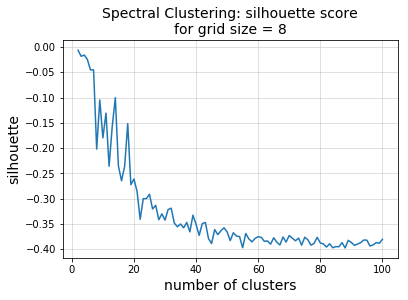
\includegraphics[width=.8\linewidth]{images/spectral_silhouette.png}
\caption{Values of the silhouette coefficient for different number of clusters. Clustering has been computed on images of size 8x8 pixels.}
\label{fig:spectral-silhouette}
\end{figure}

We tested the algorithm for all the different values of $grid\_size$ (4, 8, 16, 32, 64) and for different numbers of clusters, evaluating the results by computing the silhouette coefficient. Figure \ref{fig:spectral-silhouette} shows the performances of Spectral Clustering on images that have been undersampled to 8x8 pixels (i.e. $grid\_size = 8$). The plot shows that the silhouette has always negative values, sometimes reaching up to -0.4. A negative silhouette indicates that clusters are not well separated (rather, they overlap with each other) and that the single instances match other clusters instead of their own (i.e. they are assigned to the wrong cluster). We omitted the plots for the remaining values of $grid\_size$ as the results were pretty similar. Apparently, the structure of the clusters was not as complicated as expected, making Spectral Clustering a bad choice for the specific task. 

Let us now take a look at the results obtained by applying K-means (which is the algorithm used in the experiments) to the images. For each value of $grid\_size$ and the number of clusters $K$, we present both the Clustering Purity and the SSE curve. The latter will be used to identify the optimal value of $K$ and the former will be just a post-evaluation measure (i.e. it did not affect the choice of $K$). 

To find the \textit{elbow point} of the SSE curve, we used a technique that consists in selecting the point having the maximum distance from the line that joins the two ends of the curve itself.

Figure \ref{fig:purity} shows both the Clustering Purity and the SSE curve for different values of the parameter $grid\_size$. In each of the SSE plots we see clearly that there is a major decrease in the error until $K$ reaches a value of about 20: from that point on, the curve is not as steep as it previously was. In accordance to that, we see that our method always found the elbow point in that specific zone.

As for the Clustering Purity, in all the plots it is evident the presence of a linear, increasing trend. As the number of clusters increases, it seems that each one becomes purer and purer. This is because when we have a high number of clusters, the number of images inside them keeps decreasing along with their degree of heterogeneity. Also note that even the standard deviation keeps increasing, meaning that there are both good and bad clusters.

If we measure the Clustering Purity in the vicinity of $K=20$, we observe that its average value is around 0.1, meaning that the most frequent class in each cluster has an average frequency of 10\%. 
This is unarguably not the best result, but we have to take into account that, sometimes, images labeled with the same class may be visually different. Indeed, two images representing the same "object" can have different backgrounds, represent the object in different scales or even contain other objects. 

By clustering on raw pixels, it is difficult (if not impossible) to extract some kind of semantic information and group together images of the same class. The only goal  this type of clustering can achieve is grouping together images that are \textit{visually} similar (i.e. having the same predominant color): this is exactly what we wanted to achieve in defining LIME\#C. 

As for the undersampling techniques that we mentioned before, we used them to limit the color variety of the images to add a little bit of flexibility in defining the predominant colors.


\subsubsection{Explanation performances}

In evaluating the performances of LIME\#C we will make a comparison with both the basic version (LIME gray) and its counterpart LIME\#R , so that we will be able to judge the effectiveness of choosing visually similar images in the generation of the neighborhood rather than completely random ones. 

Figure \ref{subfig:limesharp_C_vs_sf} shows the performances of LIME\#C (compared to LIME gray) as the number of highlighted areas in the explanation increases. Similarly to the other versions of LIME, we will focus on just the case of $grid\_size = 8$ (higher values show performances that are equally bad, making them uninteresting) for all the three measures. Apart from the recall, we see that LIME\#C performs worse with respect to LIME gray under all the aspects.

\begin{figure}
\centering
\makebox[\textwidth][c]{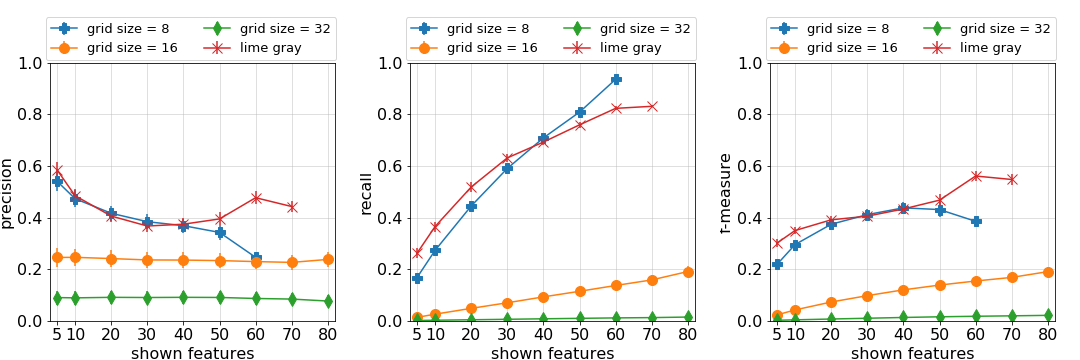
\includegraphics[width=1.1\linewidth]{images/figs/lime-sharp-C-all.png}}
\caption{LIME\#C: Precision, recall and F-measure for increasing values of the parameter $shown\_features$.}
\label{subfig:limesharp_C_vs_sf}
\end{figure}

In terms of precision, Figure \ref{subfig:R-C-comparison} shows that  LIME\#C is actually outperformed by LIME\#R: except for the first part of the plot (when $shown\_features \leq 40$) we see that it behaves worse, with a huge difference in correspondence of $shown\_features = 60$ (about 0.25 versus the $\approx 0.52$ of LIME\#R). The whole point of modifying image features (by replacing them with pieces of other images) is to identify those that, when replaced, substantially drop the veridicity of the black box's prediction and mark them as "important" (i.e. giving them a high weight in the regressor and highlighting them in the explanations). As we try to replace them with visually similar patches, the probability of disrupting the prediction is lower, causing the features not to be considered relevant.

For the recall, the differences are not so relevant: the only disadvantage of LIME\#C is that the maximum value of recall ($\approx 0.92$, reached when $shown\_features = 60$) is lower than the one of LIME\#R ($\approx 0.99$). 

\begin{figure}
\centering
\makebox[\textwidth][c]{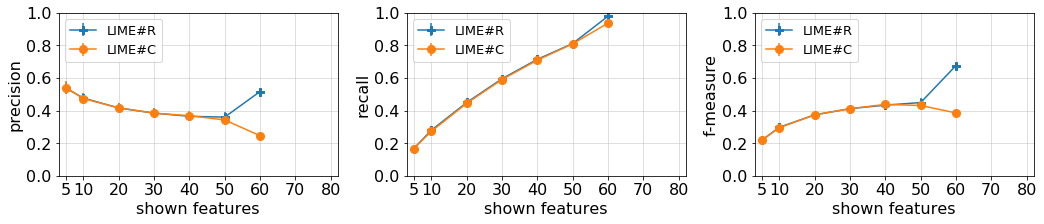
\includegraphics[width=1.1\linewidth]{images/figs/R-C-comparison.png}}
\caption{Comparison between LIME\#R and LIME\#C of precision, recall and F-measure for increasing values of the parameter $shown\_features$.}
\label{subfig:R-C-comparison}
\end{figure}

Finally, the trend of the F-measure resembles the one of the precision. Again, when $shown\_features \leq 40$, there are no relevant discrepancies between LIME\#R and LIME\#C, but for higher values we note a substantial difference: in particular, for $shown\_features = 60$, LIME\#R has an F-measure of $\approx 0.7$ while LIME\#C stops at $\approx 0.4$.
\bigskip

To conclude, let us now compare the performances of LIME\#R and LIME\#C from the point of view of the $grid\_size$ parameter (Figure \ref{fig:limesharp_C_vs_gs} in the Appendix). 

The only noticeable difference in the precision is that, when $grid\_size = 8$ and $shown\_features = 60$, LIME\#C behaves much worse than its counterpart: indeed, we have a precision of $\approx 0.25$ versus the $\approx 0.5$ of LIME\#R. This is actually consistent with what we discovered in Figure \ref{subfig:R-C-comparison}.

Figure \ref{subfig:limesharp_C_rec_vs_gs} shows that the recall follows almost the same trend as LIME\#R. The aspect that all these recall plots seem to underline is that the more we increase the grid size, the less performant the explainer is. 

Even from the point of view of the grid size, we see that the F-measure follows the trend of the precision: again, when $grid\_size = 8$ and $shown\_features = 60$, LIME\#C is outperformed by LIME\#R ($\approx 0.4$ versus $\approx 0.7$, respectively).

\newpage

\section{Overall comparison}



What emerges from the results obtained during the experiments is that high values of $grid\_size$ inevitably lead to low-quality explainers. This is because the more we reduce the size of the features, the less we are likely to capture meaningful patterns inside an image. On the other hand, lower values noticeably increase the chance of highlighting informative regions. We should however keep in mind that overly extended areas (e.g. when $grid\_size = 4$) would give rise to dispersive and coarse explanations.
To achieve meaningful results, we should limit the number of highlighted areas as well. It is then good practice to keep the value of $shown\_features$ low, because otherwise we would run the risk of detecting useless patterns outside the reference area. In Figure \ref{fig:overall-prec} we have tested the impact of increasing the value of $shown\_features$ on the explanations' precision in the newly proposed versions of LIME. In each variant, we have set $grid\_size = 8$. For low values in the range 2-20, we have witnessed how the precision drops due to the inclusion of irrelevant patterns. Similar plots for recall and F-measure are included in the Appendix (see Figure \ref{fig:overall-rec-fmea}).

\begin{figure}
\centering
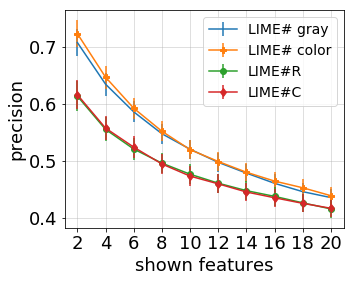
\includegraphics[width=.5\textwidth]{images/overall-figs/precision.png} 
\caption{Trend of precision for increasing values of $shown\_features$. Fixing the value of $grid\_size$ to 8, we make a comparison between the newly proposed approaches (all the "\#" variants of LIME).}
\label{fig:overall-prec}
\end{figure}

As a compromise, we now take a closer look at the performances of explanations (for all the variants of LIME\#) when $grid\_size = 8$, highlighting in each explanation from 2 to 10 features.
Table \ref{tab:overall-precision-avg} shows the value of the precision for all the versions of LIME: we fixed $grid\_size = 8$ and, among all the 1000 images in the test set, we recorded the average value and the standard deviation. With the introduction of the grid-shaped segmentation (LIME\# gray, LIME\# color) explanations tend to cover the reference area more often. About the generation of the neighborhood, instead, we see that the usage of patches from other images (LIME\#R, LIME\#C) does not bring any kind of improvement.
Table \ref{tab:overall-precision-median} shows instead the median value of the precision. The only thing to notice is that, when $shown\_features = 2$, the image-based variants perform worse than the others. Also, when $shown\_features = 8$, we see again that LIME\# gray and LIME\# color outperform the other versions.
The tables of the recall and F-measure can be found in the appendix. In those cases, the best version in terms of performances is LIME color.

\noindent
\hspace{-2mm}
\begin{table}[h]
\footnotesize
\def\arraystretch{1.3}
\begin{tabularx}{\linewidth}{ll|cccccc}
%\hline
            &    
            & \rotatebox[origin=c]{0}{\textbf{gray}}
            & \rotatebox[origin=c]{0}{\textbf{color}}     & \rotatebox[origin=c]{0}{\textbf{\# gray}}     & \rotatebox[origin=c]{0}{\textbf{\# color}}    & \rotatebox[origin=c]{0}{\textbf{\#R}}         & \rotatebox[origin=c]{0}{\textbf{\#C}}         \\
\hline
\multirow{7}{*}{\rotatebox[origin=c]{90}{\centering \textbf{Shown features}}} &&&&&&\\
& 2 & $.686 \pm .363$ & $.709 \pm .368$ & $.708 \pm .367$ & $\mathbf{.723 \pm .354}$ & $.614 \pm .388$ & $.616 \pm .388$ \\
& 3 & $.649 \pm .332$ & $.666 \pm .333$ & $\mathbf{.669 \pm .326}$ & $.681 \pm .327$ & $.579 \pm .338$ & $.583 \pm .341$ \\
& 5 & $.585 \pm .293$ & $.594 \pm .299$ & $.607 \pm .290$ & $\mathbf{.620 \pm .292}$ & $.537 \pm .298$ & $.541 \pm .297$ \\
& 8 & $.513 \pm .268$ & $.521 \pm .274$ & $.548 \pm .265$ & $\mathbf{.552 \pm .262}$ & $.496 \pm .269$ & $.495 \pm .267$ \\
& 10 & $.485 \pm .260$ & $.493 \pm .262$ & $\mathbf{.521 \pm .256}$ & $.520 \pm .255$ & $.477 \pm .260$ & $.473 \pm .257$ \\
%\hline
\end{tabularx}
\caption{Precision (mean $\pm$ standard dev.) for all the versions of LIME (for all the "\#" variants, we have set $grid\_size = 8$).}
\label{tab:overall-precision-avg}
\end{table}

\noindent
\hspace{-2mm}
\begin{table}[h]
%\footnotesize
\centering
\def\arraystretch{1.1}
\begin{tabular}{ll|cccccc}
%\hline
            &    & \rotatebox[origin=c]{0}{\textbf{gray}}      & \rotatebox[origin=c]{0}{\textbf{color}}     & \rotatebox[origin=c]{0}{\textbf{\# gray}}     & \rotatebox[origin=c]{0}{\textbf{\# color}}    & \rotatebox[origin=c]{0}{\textbf{\#R}}         & \rotatebox[origin=c]{0}{\textbf{\#C}}         \\
\hline
\multirow{7}{*}{\rotatebox[origin=c]{90}{\centering \textbf{Shown features}}} &&&&&&\\
& 2 & \textbf{1.00} & \textbf{1.00} & \textbf{1.00} &      \textbf{1.00} & .500 & .500 \\
& 3 &       .667 &        .667 &        .667 &         .667 &    .667 &    .667 \\
& 5 &       .600 &        .600 &        .600 &         .600 &    .600 &    .600 \\
& 8 &       .500 &        .500 &        \textbf{.625} &         \textbf{.625} &    .500 &    .500 \\
& 10 &       .500 &        .500 &        .500 &         .500 &    .500 &    .500 \\
%\hline
\end{tabular}
\caption{Median of the precision for all the versions of LIME (for all the "\#" variants, we have set $grid\_size = 8$).}
\label{tab:overall-precision-median}
\end{table}


\chapter{Conclusion}\label{chapt:conclusions}

In this work we have proposed an extension to the work described in \cite{lime} and deepened their idea of explanation. In particular, we have focused on the concept of interpretability of an explanation and tested the impact deriving from the usage of different shapes in the definition of images' features. Another crucial point that we have stressed was the possibility of increasing people's trust in a model just by giving them an idea of the logic behind its decision, regardless of the correctness of the outcome. This way, users can understand the causes of errors and adapt a strategy to fix them.

We have also asked ourselves what was the best way of defining neighborhood images when we do not have access to the image generation process. We have argued that replacing patches with solid colors is not a natural and convenient way of applying perturbations and proposed different solutions to approximate what would be the correct approach. For this reason, we have considered the usage of patches from other images in the neighborhood generation process and verified whether or not it was meaningful to choose visually similar features. In this regard, we have found that replacing image features with similar patterns (rather than random ones) prevents the explanation system from individuating relevant areas in the original image. The result was that explanations were less intuitive and not able to capture the representative features of each class. 

Another contribution that we have made was the definition of a measure of quality of an explanation (i.e. what is its level of comprehensibility). To do that, we have created a new annotated data set that contains a reference area (ideally, the part of the image that would be highlighted by a hypothetical optimal explanation) for each image in the test set. Referring to that information, we have also defined three measures of goodness of an explanation (from different point of views) and evaluated them on the different versions of LIME.

The peculiarity that all the variants of explainers in our approach had in common was the generation of a visual, textless explanation which only spots the areas of the image that the model looks at when performing its predictions. This perfectly makes sense in single-object recognition scenarios, where the goal is to identify the category of a unique part of the image. However, this solution turns out to be inappropriate in scene recognition challenges, where the main objective is to summarize the context of a picture based on different (and possibly unrelated) objects inside it. 

\bigskip

An interesting extension to this work would be then the generation of enriched explanations, in which different parts of an image are labeled with strings. The idea is to convince the user of the ability of the black box of recognizing scenes by giving actual proofs that support its decisions. 
As an example, suppose we teach our model to recognize pictures about classrooms: what we expect is that the black box annotates corresponding parts of the images with strings like \textit{blackboard}, \textit{teacher}, \textit{desk}, \textit{kid} and so on.

Another future research direction would be the modification of the image-based neighborhood generation process. We have seen that the usage of images which are visually similar to the one to be explained does not allow the explanation system to recognize representative features. One possible solution would be to draw both same-cluster and random images, each with a fixed probability.
Other studies might be focused instead on defining a more sophisticated neighborhood generation technique, rather than drawing instances completely at random.

Finally, an open research question is the problem of estimating the level of comprehensibility of an explanation. The problem with the method we have presented is that, for large data sets, cutting images by hand is just unfeasible as it would require huge amounts of time. The ideal solution would be a systematic approach (e.g. a mathematical formalism) that makes the whole process automatic.


\bibliographystyle{ieeetr}
\bibliography{biblio} 

\whitepage

\appendix

\chapter{Experiments results}

We attach here (for reasons of readability) the plots that show the performances of the different versions of LIME. Each of the plots is referenced and described in detail in Chapter \ref{chapt:experiments}.

\bigskip

\begin{figure}[h]
\centering
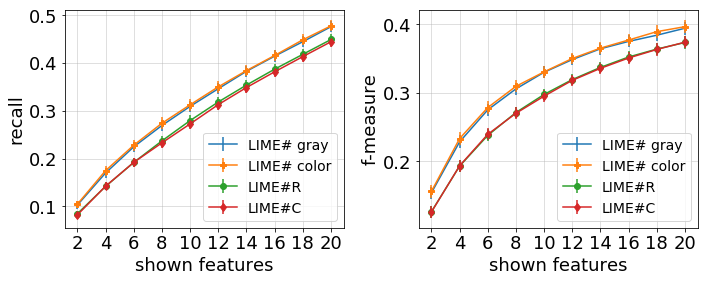
\includegraphics[width=.9\textwidth]{images/overall-figs/rec-fmea.png} 
\caption{Trends of recall and F-measure for increasing values of $shown\_features$. Fixing the value of $grid\_size$ to 8, we make a comparison between the newly proposed approaches (all the "\#" variants of LIME).}
\label{fig:overall-rec-fmea}
\end{figure}

%\section{LIME\# gray}

\begin{figure}[h]
\centering
\begin{subfigure}[b]{\linewidth}
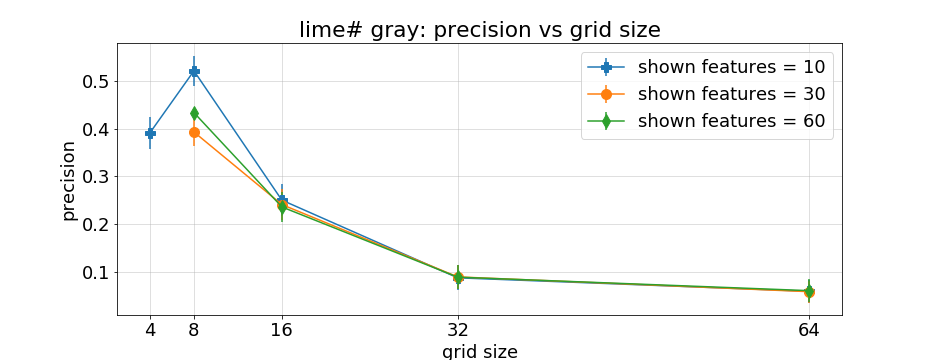
\includegraphics[width=\linewidth]{images/figs/VSGRID/limesharp gray/limesharp gray: precision vs grid size.png} 
\caption{Precision for increasing values of $grid\_size$.}
\label{subfig:limesharp_gray_prec_vs_gs}
\end{subfigure}
\begin{subfigure}[b]{\linewidth}
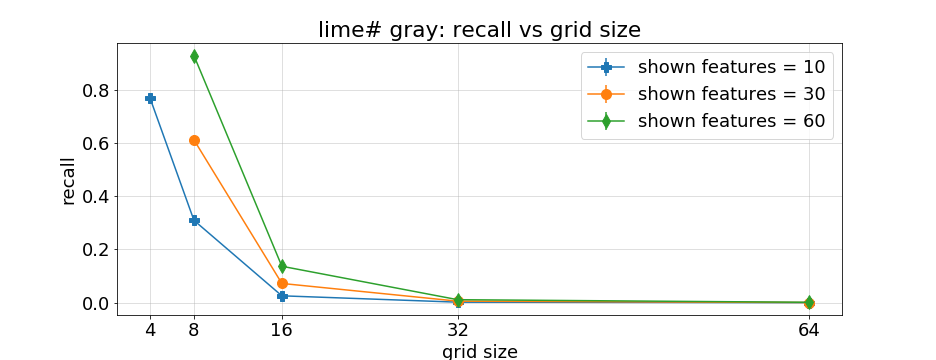
\includegraphics[width=\linewidth]{images/figs/VSGRID/limesharp gray/limesharp gray: recall vs grid size.png} 
\caption{Recall for increasing values of $grid\_size$.}
\label{subfig:limesharp_gray_rec_vs_gs}
\end{subfigure}
\begin{subfigure}[b]{\linewidth}
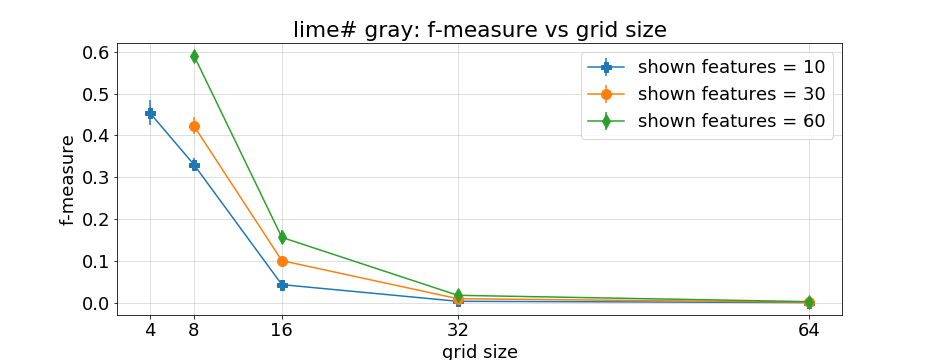
\includegraphics[width=\linewidth]{images/figs/VSGRID/limesharp gray/limesharp gray: f-measure vs grid size.png} 
\caption{F-measure for increasing values of $grid\_size$.}
\label{subfig:limesharp_gray_fmea_vs_gs}
\end{subfigure}
\caption{LIME\# gray: evaluating explanations as the grid size (in the X-axis) increases.}
\label{fig:limesharp_gray_vs_gs}
\end{figure}

\newpage

%\section{LIME\# color}

\begin{figure}[h]
\begin{subfigure}[b]{\linewidth}
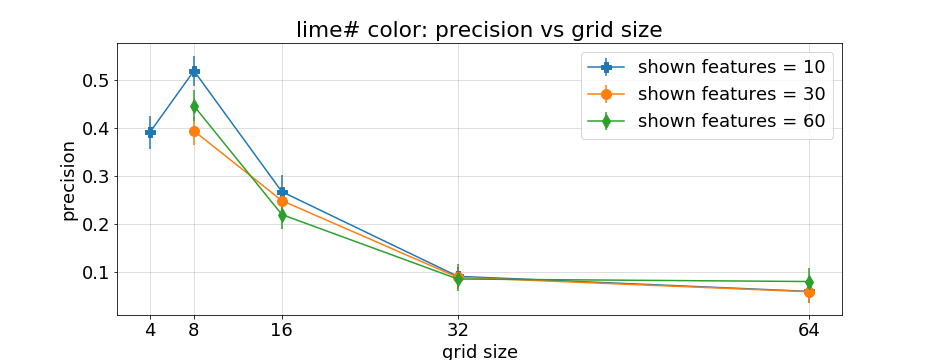
\includegraphics[width=\linewidth]{images/figs/VSGRID/limesharp color/limesharp color: precision vs grid size.png} 
\caption{Precision for increasing values of $grid\_size$.}
\label{subfig:limesharp_color_prec_vs_gs}
\end{subfigure}
\begin{subfigure}[b]{\linewidth}
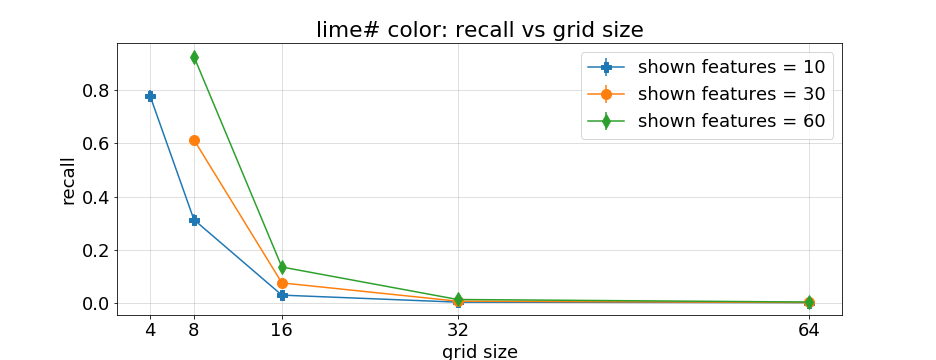
\includegraphics[width=\linewidth]{images/figs/VSGRID/limesharp color/limesharp color: recall vs grid size.png} 
\caption{Recall for increasing values of $grid\_size$.}
\label{subfig:limesharp_color_rec_vs_gs}
\end{subfigure}
\begin{subfigure}[b]{\linewidth}
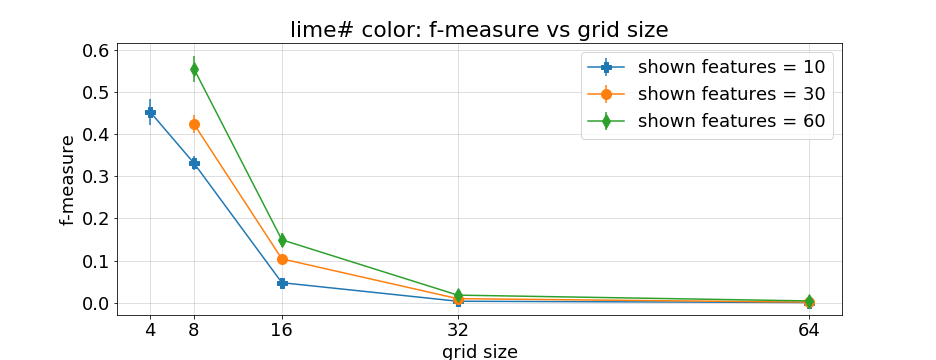
\includegraphics[width=\linewidth]{images/figs/VSGRID/limesharp color/limesharp color: f-measure vs grid size.png} 
\caption{F-measure for increasing values of $grid\_size$.}
\label{subfig:limesharp_color_fmea_vs_gs}
\end{subfigure}
\caption{LIME\# color: evaluating explanations as the grid size (in the X-axis) increases.}
\label{fig:limesharp_color_vs_gs}
\end{figure}

\newpage

%\section{LIME\#R}

\begin{figure}[h]
\begin{subfigure}[b]{\linewidth}
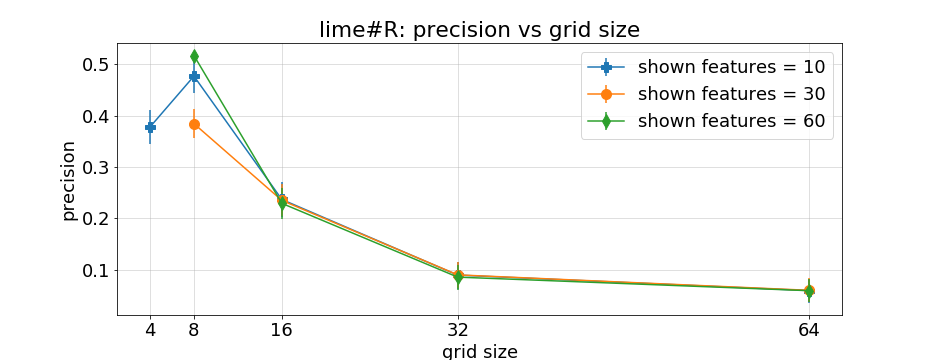
\includegraphics[width=\linewidth]{images/figs/VSGRID/limesharpR/limesharpR: precision vs grid size.png} 
\caption{Precision for increasing values of $grid\_size$.}
\label{subfig:limesharp_R_prec_vs_gs}
\end{subfigure}
\begin{subfigure}[b]{\linewidth}
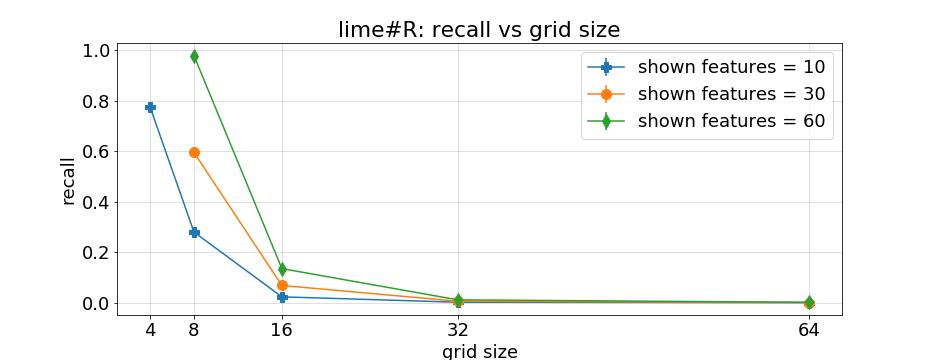
\includegraphics[width=\linewidth]{images/figs/VSGRID/limesharpR/limesharpR: recall vs grid size.png} 
\caption{Recall for increasing values of $grid\_size$.}
\label{subfig:limesharp_R_rec_vs_gs}
\end{subfigure}
\begin{subfigure}[b]{\linewidth}
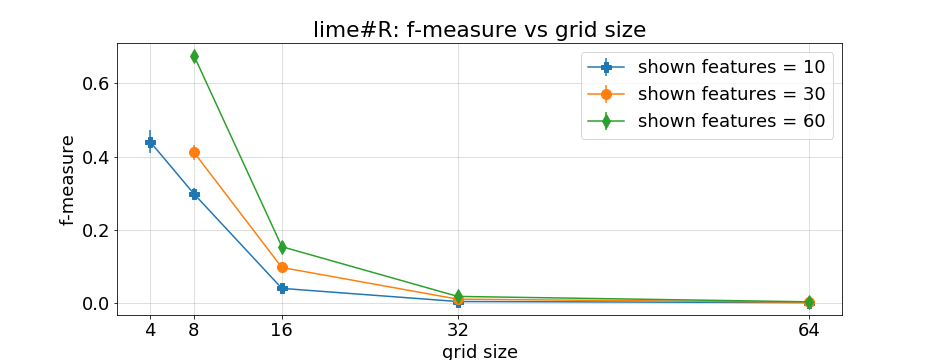
\includegraphics[width=\linewidth]{images/figs/VSGRID/limesharpR/limesharpR: f-measure vs grid size.png} 
\caption{F-measure for increasing values of $grid\_size$.}
\label{subfig:limesharp_R_fmea_vs_gs}
\end{subfigure}
\caption{LIME\#R: evaluating explanations as the grid size (in the X-axis) increases.}
\label{fig:limesharp_R_vs_gs}
\end{figure}

\newpage

%\section{LIME\#C}

\begin{figure}[h]

\begin{subfigure}[b]{\linewidth}
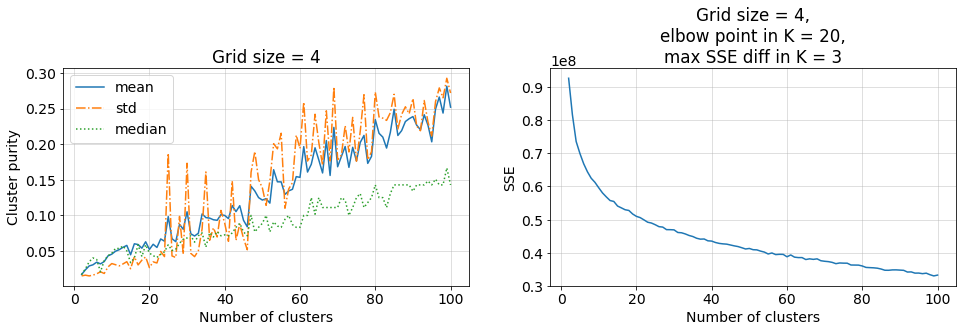
\includegraphics[width=\linewidth]{images/purity/4by4.png} 
\caption{Clustering purity and SSE curve for $grid\_size = 4$.}
\label{subfig:purity-4}
\end{subfigure}

\begin{subfigure}[b]{\linewidth}
\includegraphics[width=\linewidth]{images/purity/8by8.png} 
\caption{Clustering purity and SSE curve for $grid\_size = 8$.}
\label{subfig:purity-8}
\end{subfigure}

\begin{subfigure}[b]{\linewidth}
\includegraphics[width=\linewidth]{images/purity/16by16.png} 
\caption{Clustering purity and SSE curve for $grid\_size = 16$.}
\label{subfig:purity-16}
\end{subfigure}
\caption{Clustering Purity and SSE curve for different values of $grid\_size$. The latter is used to find the best value of the parameter K, while the former is just a post-evaluation measure.}
\end{figure}

\begin{figure}\ContinuedFloat
\begin{subfigure}[b]{\linewidth}
\includegraphics[width=\linewidth]{images/purity/32by32.png} 
\caption{Clustering purity and SSE curve for $grid\_size = 32$.}
\label{subfig:purity-32}
\end{subfigure}


\begin{subfigure}[b]{\linewidth}
\includegraphics[width=\linewidth]{images/purity/64by64.png} 
\caption{Clustering purity and SSE curve for $grid\_size = 64$.}
\label{subfig:purity-64}
\end{subfigure}
\caption{Clustering Purity and SSE curve for different values of $grid\_size$. The latter is used to find the best value of the parameter K, while the former is just a post-evaluation measure.}
\label{fig:purity}
\end{figure}


\begin{figure}[h]
\begin{subfigure}[b]{\linewidth}
\includegraphics[width=\linewidth]{images/figs/VSGRID/limesharpC/limesharpC: precision vs grid size.png} 
\caption{Precision for increasing values of $grid\_size$.}
\label{subfig:limesharp_C_prec_vs_gs}
\end{subfigure}
\begin{subfigure}[b]{\linewidth}
\includegraphics[width=\linewidth]{images/figs/VSGRID/limesharpC/limesharpC: recall vs grid size.png} 
\caption{Recall for increasing values of $grid\_size$.}
\label{subfig:limesharp_C_rec_vs_gs}
\end{subfigure}
\begin{subfigure}[b]{\linewidth}
\includegraphics[width=\linewidth]{images/figs/VSGRID/limesharpC/limesharpC: f-measure vs grid size.png} 
\caption{F-measure for increasing values of $grid\_size$.}
\label{subfig:limesharp_C_fmea_vs_gs}
\end{subfigure}
\caption{LIME\#C: evaluating explanations as the grid size (in the X-axis) increases.}
\label{fig:limesharp_C_vs_gs}
\end{figure}


%%%%%%%%%%%%%%%%%%%%%%%
% TABLES

\noindent
\hspace{-2mm}
\begin{table}[h]
\footnotesize
\def\arraystretch{1.3}
\begin{tabularx}{\linewidth}{ll|cccccc}
%\hline
            &    & \rotatebox[origin=c]{0}{\textbf{gray}}      
            & \rotatebox[origin=c]{0}{\textbf{color}}     
            & \rotatebox[origin=c]{0}{\textbf{\# gray}}     
            & \rotatebox[origin=c]{0}{\textbf{\# color}}    
            & \rotatebox[origin=c]{0}{\textbf{\#R}}         
            & \rotatebox[origin=c]{0}{\textbf{\#C}}         \\
\hline
\multirow{7}{*}{\rotatebox[origin=c]{90}{\centering \textbf{Shown features}}} &&&&&&\\
& 2 & $.150 \pm .142$ & $\mathbf{.155 \pm .141}$ & $.103 \pm .111$ & $.105 \pm .114$ & $.085 \pm .098$ & $.082 \pm .096$ \\
& 3 & $.195 \pm .164$ & $\mathbf{.200 \pm .161}$ & $.140 \pm .133$ & $.143 \pm .140$ & $.114 \pm .111$ & $.113 \pm .114$ \\
& 5 & $.262 \pm .184$ & $\mathbf{.264 \pm .179}$ & $.198 \pm .155$ & $.203 \pm .164$ & $.167 \pm .135$ & $.167 \pm .138$ \\
& 8 & $.326 \pm .192$ & $\mathbf{.331 \pm .186}$ & $.269 \pm .172$ & $.274 \pm .180$ & $.237 \pm .160$ & $.233 \pm .154$ \\
& 10 & $.365 \pm .192$ & $\mathbf{.369 \pm .184}$ & $.309 \pm .174$ & $.313 \pm .183$ & $.280 \pm .166$ & $.273 \pm .157$ \\
%\hline
\end{tabularx}
\caption{Recall (mean $\pm$ standard dev.) for all the versions of LIME (for all the "\#" variants, we have set $grid\_size = 8$).}
\label{tab:overall-recall-avg}
\end{table}

%\bigskip

\noindent
\hspace{-2mm}
\begin{table}[h]
\centering
%\footnotesize
\def\arraystretch{1.3}
\begin{tabular}{ll|cccccc}
%\hline
            &    & \rotatebox[origin=c]{0}{\textbf{gray}}      
            & \rotatebox[origin=c]{0}{\textbf{color}}     
            & \rotatebox[origin=c]{0}{\textbf{\# gray}}     
            & \rotatebox[origin=c]{0}{\textbf{\# color}}    
            & \rotatebox[origin=c]{0}{\textbf{\#R}}         
            & \rotatebox[origin=c]{0}{\textbf{\#C}}         \\
\hline
\multirow{7}{*}{\rotatebox[origin=c]{90}{\centering \textbf{Shown features}}} &&&&&&\\
& 2 &       .109 &        \textbf{.113} &        .068 &         .067 &    .057 &    .054 \\
& 3 &       .147 &        \textbf{.153} &        .096 &         .095 &    .083 &    .080 \\
& 5 &       .211 &        \textbf{.216} &        .148 &         .149 &    .126 &    .125 \\
& 8 &       .281 &        \textbf{.284} &        .220 &         .218 &    .192 &    .186 \\
& 10 &       .322 &        \textbf{.327} &        .261 &         .256 &    .231 &    .225 \\
%\hline
\end{tabular}
\caption{Median of the recall for all the versions of LIME (for all the "\#" variants, we have set $grid\_size = 8$).}
\label{tab:overall-recall-median}
\end{table}

\newpage

\noindent
\hspace{-2mm}
\begin{table}[h]
\footnotesize
\def\arraystretch{1.3}
\begin{tabularx}{\linewidth}{ll|cccccc}
%\hline
            &    & \rotatebox[origin=c]{0}{\textbf{gray}}      
            & \rotatebox[origin=c]{0}{\textbf{color}}     
            & \rotatebox[origin=c]{0}{\textbf{\# gray}}     
            & \rotatebox[origin=c]{0}{\textbf{\# color}}    
            & \rotatebox[origin=c]{0}{\textbf{\#R}}         
            & \rotatebox[origin=c]{0}{\textbf{\#C}}         \\
\hline
\multirow{7}{*}{\rotatebox[origin=c]{90}{\centering \textbf{Shown features}}} &&&&&&\\
&  2 & $.202 \pm .165$ & $\mathbf{.210 \pm .169}$ & $.154 \pm .139$ & $.156 \pm .138$ & $.127 \pm .127$ & $.126 \pm .127$ \\
&  3 & $.249 \pm .171$ & $\mathbf{.257 \pm .172}$ & $.198 \pm .146$ & $.201 \pm .149$ & $.163 \pm .129$ & $.163 \pm .131$ \\
&  5 & $.301 \pm .160$ & $\mathbf{.307 \pm .164}$ & $.254 \pm .141$ & $.259 \pm .144$ & $.218 \pm .133$ & $.218 \pm .131$ \\
&  8 & $.334 \pm .150$ & $\mathbf{.340 \pm .150}$ & $.306 \pm .131$ & $.310 \pm .133$ & $.271 \pm .129$ & $.270 \pm .128$ \\
& 10 & $.350 \pm .148$ & $\mathbf{.356 \pm .146}$ & $.330 \pm .127$ & $.331 \pm .129$ & $.298 \pm .127$ & $.295 \pm .124$ \\
%\hline
\end{tabularx}
\caption{F-measure (mean $\pm$ standard dev.) for all the versions of LIME (for all the "\#" variants, we have set $grid\_size = 8$).}
\label{tab:overall-fmeasure-avg}
\end{table}

\noindent
\hspace{-2mm}
\begin{table}[h]
%\footnotesize
\centering
\def\arraystretch{1.3}
\begin{tabular}{ll|cccccc}
%\hline
            &    & \rotatebox[origin=c]{0}{\textbf{gray}}      
            & \rotatebox[origin=c]{0}{\textbf{color}}     
            & \rotatebox[origin=c]{0}{\textbf{\# gray}}     
            & \rotatebox[origin=c]{0}{\textbf{\# color}}    
            & \rotatebox[origin=c]{0}{\textbf{\#R}}         
            & \rotatebox[origin=c]{0}{\textbf{\#C}}         \\
\hline
\multirow{7}{*}{\rotatebox[origin=c]{90}{\centering \textbf{Shown features}}} &&&&&&\\
& 2 &       .169 &        \textbf{.177} &        .120 &         .120 &    .098 &    .097 \\
& 3 &       .222 &        \textbf{.233} &        .165 &         .164 &    .139 &    .138 \\
& 5 &       .293 &        \textbf{.299} &        .232 &         .235 &    .198 &    .198 \\
& 8 &       .336 &        \textbf{.347} &        .295 &         .299 &    .265 &    .260 \\
& 10 &       .360 &        \textbf{.365} &        .329 &         .329 &    .301 &    .296 \\
%\hline
\end{tabular}
\caption{Median of the F-measure for all the versions of LIME (for all the "\#" variants, we have set $grid\_size = 8$).}
\label{tab:overall-fmeasure-median}
\end{table}


\end{document}
